%
%
\chapter{Térmica}


\begin{enumerate}[start=1,label={\bfseries Q\arabic*.}]


\item A otimização de um processo termodinâmico envolve a avaliação de duas etapas consecutivas:


\item[(1)] A compressão de $n$ $moles$ de um gás ideal diatômico ($\gamma = 1,4$ e $C_{V} = 5R/2$, onde $R = 8,31 \ J/mol \cdot K$ é a constante universal dos gases), inicialmente à pressão $P_{0} = 1,01 \times 10^{5} \ N/m^{2}$, temperatura $T_{0} = 330 \ K$ e volume $V_{0} = 1,00 \ l$, para um volume final de $100 \ ml$.

\item[(2)] A subsequente exaustão de uma fração do gás para que sua pressão retorne ao valor inicial $P_{0}$, porém à temperatura de $300 \ K$.

    A avaliação consiste na comparação entre os casos em que a compressão (1) é isotérmica ou adiabática. Considere, se necessário, que $10^{1,3} \approx 20$, $10^{1,4} \approx 25$ e $10^{1,7} \approx 50$.

a) Para o caso isotérmico, determine a pressão logo após a compressão.

{\color{red}

No caso isotérmico

$$
P_{0} V_{0} = P_{f} V_{f} \quad \Rightarrow \quad P_{f} = 10 P_{0} = 10,1 \times 10^{5} N/m^{2}.
$$

}

b) Para o caso adiabático, determine a pressão logo após a compressão.

{\color{red}

No caso adiabático

$$
P_{0} V_{0}^{\gamma} = P_{f} V_{f}^{\gamma} \quad \Rightarrow \quad P_{f} = 10^{\gamma} P_{0} = 10^{1,4} P_{0} \approx 25,3 \times 10^{5} N/m^{2}.
$$

}

c) Determine a fração do gás inicial que é liberada na etapa (2).
{\color{red}

O número de moles ao final da compressão é o mesmo em ambos os casos porque as variáveis de estado são as mesmas. O número de moles inicial era, da equação do gás ideal,

$$
n = \frac{P_{0}V_{0}}{RT_{0}}.
$$

Após a exaustão, com $T_{2} = 300 \ K$, o número de moles será

$$
n^{\prime} = \frac{P_{0}V_{0}}{RT_{0}}.
$$


Portanto,

$$
\frac{n^{\prime}}{n} = \frac{T_{0}V_{f}}{T_{2}V_{0}} = \frac{330 \prime 0,1}{300 \prime 1} = 0,11.
$$

e conclui-se que uma fração de 0,89 do gás inicial é liberada (ou $89\%$).

}

d) Esboce as duas etapas de compressão (isotérmica e adiabática) em um diagrama $P \times V$ e
determine em qual delas o trabalho realizado sobre o gás é menor.

{\color{red}

Um esboço dos dois processos pode ser visto na figura abaixo.

\begin{figure}[H]
  \centering
  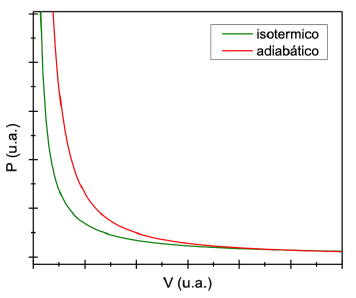
\includegraphics[scale=0.5]{termica-img/isoter.png}
%  \caption{}\label{}
\end{figure}

Como o trabalho realizado (em módulo) é a área sob a curva, é óbvio que ele é menor no caso isotérmico. Alternativamente, pode-se calcular os dois trabalhos. No caso isotérmico

$$
W_{\text{isoter}} = -n R T_{0} \int_{V_{0}}^{V_{f}} \frac{d V}{V} = -P_{0} V_{0} \ln \left(\frac{V_{f}}{V_{0}}\right) = 101 \ln 10 \approx 233 \mathrm{J}
$$

No caso adiabático


\begin{eqnarray*}
W_{\text{adia}} &=& -P_{0} V_{0}^{\gamma} \int_{V_{0}}^{V_{f}} \frac{d V}{V^{\gamma}}=\frac{1}{\gamma-1} P_{0} V_{0}^{\gamma}\left[V_{f}^{(1-\gamma)}-V_{0}^{(1-\gamma)}\right]=\frac{1}{\gamma-1} P_{0} V_{0}\left[\left(\frac{V_{0}}{V_{f}}\right)^{(\gamma-1)}-1\right] \\
&=& 2,5 \times 101 \times\left(10^{0,4}-1\right)=2,5 \times 101 \times\left(\frac{10^{1,4}}{10}-1\right) \approx 380 \mathrm{J}
\end{eqnarray*}


}




\item A figura abaixo ilustra dois compartimentos separados por uma válvula. O compartimento da esquerda, de volume $V_{0}$, contém 2 moles de um gás ideal na pressão $P_{0}$. O compartimento da direita, de volume $4V_{0}$, está inicialmente vazio. Ao abrir a válvula, o gás sofre uma expansão livre (adiabática e sem realização de trabalho) e passa a ocupar os dois compartimentos.

\begin{figure}[H]
  \centering
  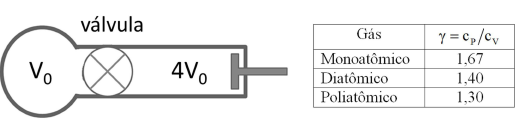
\includegraphics[scale=0.5]{termica-img/tubo.png}
%  \caption{}\label{}
\end{figure}


  a) Qual é a pressão dos gás após a expansão livre?

  \resposta

  b) Determine a variação da entropia do gás no processo de expansão livre.

  \resposta

  c) Após a expansão livre, o gás é comprimido num processo adeibático e quase-estático até o volume inicial $V_{0}$. Ao final desse processo, a pressão do gás é $P = 5^{2/5} P_{0}$. O gás é monoatônico, diatômico ou poliatômico?

  \resposta

  d) Determine a razão $U_{f}/ U_{i}$ entre a energia interna final, $U_{f}$ (após a compressão), e a incial, $U_{i}$ (antes da expansão livre).





\item Uma amostra de 1,0 mol de gás ideal monoatômico (capacidades térmicas molares $C_{v} = 3R/2$ e $C_{p} = 5R/2$) é submetida ao processo termodinâmico cíclico mostrado no diagrama de pressão versus volume da figura abaixo. O ciclo é percorrido no sentido horário. As pressões e os volumes nos pontos A,B e C são mostrados na figura e todas as transformações sofridas pelo gás são reversíveis, seguindo as linhas retas contínuas AB, BC e CA. Dê suas respostas em termos da constante universal dos gases $R$ e da pressão $P_{i}$ e do volume $V_{i}$ do gás no ponto A.

\begin{figure}
  \centering
  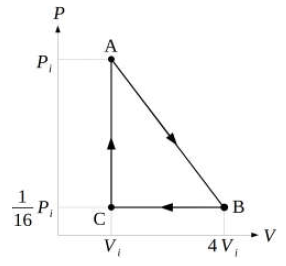
\includegraphics[scale=1]{termica-img/gas.png}
%  \caption{}\label{}
\end{figure}


  a) Encontre as temperaturas $T_{A}$, $T_{B}$ e $T_{C}$ do gás nos pontos A, B e C.

\resposta A partir da equação dos gases ideais, $PV = nRT$, com $n = 1\ mol$, temos
$$
\begin{aligned}
P_{A} V_{A} &=R T_{A} \quad \Rightarrow \quad T_{A}=\frac{P_{i} V_{i}}{R} \\
P_{B} V_{B} &=R T_{B} \quad \Rightarrow \quad T_{B}=\frac{P_{i} V_{i}}{4 R} \\
P_{C} V_{C} &=R T_{C} \quad \Rightarrow \quad T_{C}=\frac{P_{i} V_{i}}{16 R}
\end{aligned}
$$


b) Encontre o calor total trocado entre a vizinhança e o gás a cada ciclo, $Q_{ciclo}$.

\resposta Como a energia interna do gás é uma função de estado, sua variação ao longo de um ciclo é nula. Por outro lado, essa variação é a soma do trabalho líquido $W_{ciclo}$ realizado pela vizinhança sobre o gás com a transferência líquida $Q_{ciclo}$ de energia na forma de calor da vizinhança para
o gás. Portanto,
$$
Q_{ciclo} = - W_{ciclo}
$$
O trabalho líquido $W_{ciclo}$ é igual à área delimitada pelo gráfico do ciclo. Logo,
$$
Q_{\text {ciclo }}=\frac{1}{2}\left(P_{A}-P_{C}\right)\left(V_{B}-V_{A}\right) \quad \Rightarrow \quad Q_{\text {ciclo }}=\frac{45}{32} P_{i} V_{i}
$$




c) Calcule o calor trocado entre a vizinhança e o gás entre os pontos A e B, $Q_{AB}$.

\resposta Como se trata de um mol de gás ideal monoatômico, fazendo uso da primeira lei da termodinâmica,
$$
\Delta U_{A B}=W_{A B}+Q_{A B}
$$
$$
\Delta U_{A B}=\frac{3}{2} R\left(T_{B}-T_{A}\right)=-\frac{9}{8} P_{i} V_{i}
$$
e
$$
W_{A B}=-\int_{A \rightarrow B} P d V=-\frac{1}{2}\left(P_{B}+P_{A}\right)\left(V_{B}-V_{A}\right)=-\frac{51}{32} P_{i} V_{i}
$$



d) Calcule a variação da entropia do gás entre os pontos A e B, $\Delta S_{AB} = S_{B} - S_{A}$.

\resposta Como a entropia do gás é função de estado, sua variação entre os pontos $A$ e $B$ pode ser calculada ao longo de qualquer caminho que os conecte. Vamos efetuar o cálculo ao longo da combinação dos trechos retilíneos $AC$ e $CB$. No primeiro trecho, correspondente a uma transformação isovolumétrica, temos
$$
\Delta S_{A C}=\int_{A \rightarrow C} \frac{d Q}{T}=\int_{T_{A}}^{T_{C}} \frac{C_{V} d T}{T}=\frac{3}{2} R \ln \frac{T_{C}}{T_{A}}=-\frac{3}{2} R \ln (16)
$$
em que $C_{V} = (3/2)R$ é a capacidade térmica a volume constante de um mol de gás ideal monoatômico. No segundo trecho, correspondente a uma transformação isobárica, temos
$$
\Delta S_{C B}=\int_{C \rightarrow B} \frac{d Q}{T}=\int_{T_{C}}^{T_{B}} \frac{C_{P} d T}{T}=\frac{5}{2} R \ln \frac{T_{B}}{T_{C}}=\frac{5}{2} R \ln (4)
$$
em que $C_{P} = (5/2)R$ é a capacidade térmica a pressão constante de um mol de gás ideal monoatômico. Combinando esses dois resultados, obtemos
$$\begin{array}{c}
\Delta S_{A B}=\Delta S_{A C}+\Delta S_{C B}=\frac{5}{2} R \ln (4)-\frac{3}{2} R \ln (16) \\
\Delta S_{A B}=-R \ln (2)<0
\end{array}$$





\item Uma região cilíndrica de seção transversal $A = 5 \times 10^{-3} \ m^{2}$ e cujo comprimento é inicialmente $L = 25 \ cm$ é ocupada por $5 \times 10^{-3} m^{2} \ mol$ de um gás monoatômico ideal ($c_{V} = 3R/2 = 12,5 \ Jmol^{-1} K^{-1}$). Uma das bases do cilindro é um êmbolo móvel sem atrito acoplado a uma mola de constante elástica $400 \ N/cm$ inicialmente não deformada e fixa num antepara imóvel, como mostrado na figura. O gás está em equilíbrio, isolado termicamente, a uma temperatura de $300 \ K$ e uma pressão externa de $1 \ atm = 1 \times 10^{5} \ N/m^{2}$. Fornece-se então quase-estaticamente uma certa quantidade de calor $Q$ ao gás e ele se expande, empurrando o êmbolo e comprimindo a mola de $2 \ cm$.


\begin{figure}
  \centering
  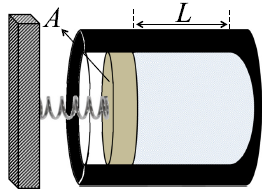
\includegraphics[scale=0.8]{termica-img/embolo.png}
%  \caption{}\label{}
\end{figure}


  a) Determine a pressão final do gás.

  \resposta

  b) Determine a temperatura final do gás.

  \resposta

  c) Determine o trabalho realizado pelo gás.

  \resposta

  d) Determine o calor $Q$ fornecido ao gás.

  \resposta





\item Um tubo em forma de U (figura à \textit{esquerda}) com seção transversal de área de $20 \ cm^{2}$ e paredes diatérmicas (isto é, que permitem a passagem de calor) contém água (região cinza, densidade de $1,0 \times 10^{3} \ kg/m^{3}$) e encontra-se aberto em suas extremidades à pressão atmosférica de aproximadamente $1,0 \times 10^{5} N/m^{2}$ e a uma temperatura de $3,0 \times 10^{2} \ K$, conforme a figura. Na extremidade direita, um êmbolo móvel, impermeável, sem atrito com as paredes e de espessura e massa desprezíveis é ajustado na superfície do líquido. A boca da outra extremidade é então vedada, aprisionando uma coluna de ar de altura $L_{i} 5,0 \ cm$. Um líquido denso X (região preta) é introduzido lentamente sobre o êmbolo, empurrado-o para baixo e, consequentemente, comprimindo o ar confinado na outra extremidade em temperatura constante (figura à \textit{direita}). Quando a altura da coluna do líquido X é $H = 5,0 \ cm$, a altura da coluna de ar na outra extremidade é $L_{f} = 4,5 \ cm$. Suponha que o ar se comporte como um gás ideal.

\begin{figure}[H]
  \centering
  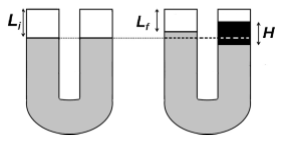
\includegraphics[scale=1]{termica-img/tubo2.png}
\end{figure}


a) Qual é a pressão na coluna de ar aprisionado após a compressão?

\resposta

b) Qual foi o trabalho realizado sobre o ar aprisionado?

\resposta

c) Qual foi a quantidade de calor trocada entre o ar aprisionado e o ambiente?

\resposta

d) Ache a densidade do líquido X.

\resposta





\item Um estudante quer determinar o calor específico $c_{x}$ de uma substância $x$ desconhecida. Para isso, dispõe de um calorímetro, que é um dispositivo que idealmente não troca calor com o ambiente. A capacidade térmica $K$ do calorímetro é conhecida. O calorímetro encontra-se inicialmente à temperatura ambiente $T_{amb}$. O procedimento experimental adotado consiste em colocar uma massa conhecida de água $m_{H_{2}O}$ à temperatura ambiente $T_{amb}$ no calorímetro, adicionar uma massa conhecida da substância $x$, $m_{x}$, inicialmente a uma temperatura $T_{x} > T_{amb}$ e medir a temperatura final de equilíbrio $T_{eq}$. Se necessário, use $\sqrt{2} \cong 1,4$ e $\sqrt{26} \cong 5,1$.


a) Escreva a equação necessária para obter $c_{x}$ a partir das grandezas fornecidas.

\resposta A conservação de energia interna leva a
$$
m_{x} c_{x}\left(T_{x}-T_{e q}\right)=\left(K+m_{H_{2} O} c_{H_{2} O}\right)\left(T_{e q}-T_{a m b}\right) \Rightarrow c_{x}=\frac{\left(K+m_{H_{2} O C_{H_{2} O}}\right)\left(T_{e q}-T_{a m b}\right)}{m_{x}\left(T_{x}-T_{e q}\right)}
$$


b) Considerando $K = 30,0 cal/ºC$, o calor específico da água $c_{H_{2}O} = 1,0 cal/(g ºC)$ e utilizando $m_{H_{2}O} = 50,0 g$, $m_{x} = 200 g$, $T_{x} = 37,8 ºC$, $T_{amb} = 25,0 \pm 0,1 ºC$, o estudante determinou que a temperatura final de equilíbrio do sistema foi de $T_{eq} = 27,8 \pm 0,1 ºC$. Calcule $c_{x}$. Expresse seu resultado com o erro associado ao valor de $c_{x}$.

\resposta (b) Usando os dados fornecidos e as fórmulas de propagação de erros do formulário
$$
\begin{aligned}
c_{x} &=\frac{(30,0+50,0 \times 1,0)(27,8 \pm 0,1-25,0 \pm 0,1)}{200(37,8-27,8 \pm 0,1)} \\
&=0,40 \times \frac{2,8 \pm 0,14}{10,0 \pm 0,1}
\end{aligned}
$$
A fração acima é
$$
\frac{2,8 \pm 0,14}{10,0 \pm 0,1}=0,28[1 \pm \sqrt{\left(\frac{0,14}{2,8}\right)^{2}+\left(\frac{0,1}{10,0}\right)^{2}}]
$$
$$
\begin{array}{l}
=0,28[1 \pm \sqrt{25 \times 10^{-4}+10^{-4}}] \\
=0,28[1 \pm \sqrt{26 \times 10^{-4}}] \\
=0,28\left[1 \pm 5,1 \times 10^{-2}\right] \\
=0,28 \pm 0,014
\end{array}
$$
Finalmente,
$$
c_{x}=0,40 \times(0,28 \pm 0,014)
$$
$$
c_{x}=(0,112 \pm 0,006) \text { cal/ }\left(\mathrm{g}^{\circ} \mathrm{C}\right)
$$




\item O motor de Stirling é uma máquina térmica cujo ciclo é composto por dois processos isotérmicos e dois processos isocóricos (isovolumétricos). Considere que $1 \ mol$ de um gás monoatômico ideal ($C_{V} = 3R/2$) atravesse um ciclo de Stirling formado pelos seguintes processos consecutivos:


\item[(1)] compressão isotérmica até $1/3$ do volume inicial $V_{0}$ à temperatura $T_{0}$;
\item[(2)] aquecimento a volume constante até o dobro da temperatura inicial $T_{0}$;
\item[(3)] expansão isotérmica até o volume inicial $V_{0}$;
\item[(4)] resfriamento isovolumétrico até a temperatura inicial $T_{0}$.



a) Esboce o ciclo acima num diagrama $P \times V$ (pressão por volume).
b) Determine a variação da energia interna do gás nos processos 1 e 2 em termos de $R$ e $T_{0}$.
c) Determine o trabalho realizado pelo gás no processo 3 em termos de $R$ e $T_{0}$.
d) Determine o rendimento dessa máquina.




\item Considere uma máquina de Carnot operando com um paramagneto ideal, cuja equação de estado é dada pela lei de Curie

$$
M = D \frac{H}{T},
$$
sendo $M$ a magnetização, $H$ o campo magnético, $T$ a temperatura e $D$ uma constante. A variação de energia interna é dada em termos da variação da entropia e da magnetização por $dU = T \ dS + H \ dM$ (o termo $HdM$ é análogo ao termo $-PdV$ para o gás ideal), e vale também que $dU = C_{M}dT$, com $C_{M}$ constante.


a) Determine a relação que vincula os valores iniciais da magnetização e da temperatura $M_{i}$, $T_{i}$ aos valores finais $M_{f}$ , $T_{f}$ em uma transformação adiabática, em termos de $C_{M}$ e $D$.

b) Represente o ciclo, composto por duas transformações adiabáticas e duas transformações isotérmicas, em um diagrama $H-M$. As isotermas correspondem respectivamente a uma temperatura mais alta, $T_{Q}$, e outra mais baixa, $T_{F}$. Indique os quatro estados nos vértices do diagrama como ($M_{1},H_{1}$) (início do ciclo, no valor mais alto para a magnetização e à temperatura $T_{Q}$), ($M_{2},H_{2}$), ($M_{3},H_{3}$), ($M_{4},H_{4}$).

c) Calcule o trabalho total realizado no ciclo, em função de $M_{1}$, $M_{2}$, $T_{Q}$, $T_{F}$ e da constante $D$.

d) Obtenha a eficiência do ciclo, dada pela razão entre o trabalho total realizado e o calor absorvido (à temperatura $T_{Q}$).





\item Uma máquina térmica de um gás ideal monoatômico funciona de acordo com um ciclo que tem inicialmente uma expansão adiabática partindo de um estado $A$ de volume $V_{0}$ até um estado $B$ cujo volume é $rV_{0}$ (com $r > 1$). O processo é seguido por uma contração isotérmica de $B$ até o estado $C$, que possui o mesmo volume de $A$. Finalmente, o ciclo se completa por uma compressão isovolumétrica de $C$ até $A$.


 a) Represente no diagrama $P - V$ o ciclo realizado por esta máquina térmica.

 \resposta O gráfico pedido é mostrado na Fig. \ref{diagramapvpng}:
 \begin{figure}[H]
   \centering
   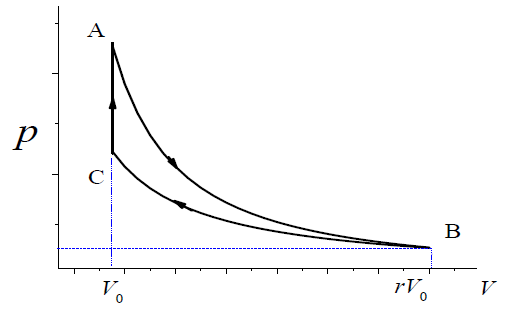
\includegraphics[scale=1]{termica-img/diagramapv.png}
   \caption{Gráfico esquemático mostrando o ciclo num diagrama $p \times V$}\label{diagramapvpng}
 \end{figure}


b) Calcule (i) o trabalho total realizado pelo gás e (ii) o calor injetado no gás, ambos durante um ciclo completo. Deixe sua resposta em função de $r$, $\gamma \equiv c_{P} /c_{V}$ e das temperaturas extremas $T_{max}$ e $T_{min}$, que são, respectivamente, as temperaturas máxima e mínima entre as quais o ciclo opera. Lembre-se de que $c_{P} - c_{V} = R$.

\resposta (i) De maneira geral, o trabalho realizado pelo gás num processo reversível quando o volume varia de $V_{1}$ até $V_{2}$ é dado por
%
\begin{equation}
  W = \int_{V_{1}}^{V_{2}} p dV
\end{equation}
%
Portanto, o trabalho realizado no trecho CA é nulo, pois não há variação de volume. O trecho $AB$ é adiabático, portanto não há troca de calor $Q_{AB}$ entre o gás e a vizinhança. Da primeira lei da termodinâmica $ \Delta U = Q - W $ ($U$ é a energia interna),
%
\begin{equation}
  W_{AB} = - \Delta U_{AB} = nc_{V} (T_{A} - T_{B}) ,
\end{equation}
%
onde usamos a express~ao para a energia interna de um gás ideal. Finalmente, na isoterma $BC$, usando a equação de estado do gás ideal,
%
\begin{equation}
  W_{BC} = \int_{rV_{o}}^{V_{o}} p dV = - n R T_{B} ln r .
\end{equation}
%
Como $T_{C} = T_{B}$ e as isotermas são hipérboles $ p = n R T / V $ num gráfico $p \times V$, segue que $T_{min} = T_{B} < T_{A} = T_{max}$. Logo, usando $c_{V} = R/ (\gamma - 1) $, o trabalho total é dado por
%
\begin{equation}
  W_{total} = \frac{nR}{\gamma - 1} (T_{max} - T_{min}) - n R T_{min} \mbox{ln} r .
\end{equation}
%
(ii) Só há troca de calor entre o gás e a vizinhança nos trechos $BC$ e $CA$, pois o processo $AB$ é adiabático. Como $BC$ é uma isoterma, a energia interna do gás se mantém constante e, usando a primeira lei,
%
\begin{equation}
  Q_{BC} = W_{BC} = -nRT_{B} \mbox{ln} r < 0 ,
\end{equation}
%
o que corresponde a uma liberação de calor do gás para sua vizinhança. Na isocórica $CA$, o trabalho é nulo e, usando novamente a primeira lei,
%
\begin{equation}
  Q_{CA} = \Delta U_{CA} = nc_{V} (T_{A} - T_{C}) = n c_{V} (T_{max} - T_{min}) .
\end{equation}
%
Portanto, o calor injetado no gás é
%
\begin{equation}
  Q_{injetado} = \frac{nR}{\gamma - 1} (T_{max} - T_{min}) .
\end{equation}
%



c) Determine o rendimento do ciclo.

\resposta O rendimento é dado por
%
\begin{equation}
  \eta = \frac{W_{total}}{Q_{injetado}} = 1 - \frac{ (\gamma - 1) T_{min} }{T_{max} - T_{min}} \mbox{ln} r .
\end{equation}
%


 d) Escreva o rendimento do ciclo apenas em função de $T_{max}$ e $T_{min}$ (caso já não o tenha feito no item (c)). Considere o caso em que $T_{max} = 2T_{min} > 0$. Determine a razão entre o rendimento desta máquina e o rendimento de um ciclo de Carnot. Qual tem o maior rendimento? Isso faz sentido com o que se espera da segunda lei da termodinâmica? Justifique sua resposta.

\resposta Na adiabática $AB$ temos que
%
\begin{equation}
  p_{A} V_{o}^{\gamma} = p_{B} (r V_{o})^{\gamma} \Rightarrow p_{B} = p_{A} / r^{\gamma} ,
\end{equation}
%
e na isoterma $BC$ temos que
%
\begin{equation}
  p_{B} r V_{o} = p_{C} V_{o} \Rightarrow p_{C} = r p_{B} ,
\end{equation}
%
donde
%
\begin{equation}
  r = \frac{p_{C}}{p_{B}} = \frac{p_{C}}{p_{A}} r^{\gamma} \Rightarrow r^{\gamma - 1} = \frac{p_{A}}{p_{C}} .
\end{equation}
%
Da equação de estado dos gases ideais para a isovolumétrica $CA$
%
\begin{equation}
  \frac{p_{A}}{p_{C}} = \frac{T_{A}}{T_{C}} = \frac{T_{max}}{T_{min}} .
\end{equation}
%
Assim,
%
\begin{equation}
  r = \left( \frac{T_{max}}{T_{min}}   \right)^{1/(\gamma - 1)}
\end{equation}
%
Levando na expressão para o rendimento,
%
\begin{equation}
  n = 1 - \frac{T_{min}}{(T_{max} - T_{min})} \mbox{ln} \left( \frac{T_{max}}{T_{min}} \right) .
\end{equation}
%
Se $T_{max} = 2T_{min}$, temos que
%
\begin{equation}
  \eta = 1 - \mbox{ln} 2 \approx 0.31 ,
\end{equation}
%
e o rendimento da máquina de Carnot correspondente é
%
\begin{equation}
  \eta_{Carnot} = 1 - \frac{T_{min}}{T_{max}} = 0.5 ,
\end{equation}
%
de forma que
%
\begin{equation}
  \frac{\eta}{\eta_{Carnot}} = 2 (1 - \mbox{ln}2 ) .
\end{equation}
%
O rendimento da máquina é menor do que o da máquina de Carnot correspondente. Isso é o esperado porque uma das consequências da segunda lei da termodinâmica é que nenhuma máquina operando entre dois reservatórios a temperaturas $T_{max}$ e $T_{min}$ pode ter rendimento maior que a máquina de Carnot entre esses reservatórios.









\item Um gás ideal contido num recipiente, inicialmente com volume $V_{A}$ e pressão $p_{A}$ (estado $A$), sofre expansão isobárica até atingir o volume $V_{B}$ (estado $B$). O gás sofre então uma expansão adiabática, até que sua pressão seja $p_{C}$ (estado $C$), de forma que uma contração isobárica (até o estado $D$) seguida de uma compressão adiabática levem o gás novamente à situação inicial (estado $A$). Considere dada a razão entre os calores específicos do gás a pressão constante e a volume constante.


a) Represente as transformações descritas acima em um diagrama $p-V$, indicando os estados $A$, $B$, $C$ e $D$.
b) Calcule o calor trocado em cada trecho do ciclo, em termos de $p_{A}$, $V_{A}$, $V_{B}$, $p_{C}$ e $\gamma$.
c) Determine a eficiência do ciclo, isto é, a razão entre o trabalho realizado pelo gás e o calor absorvido por ele.



\item Um recipiente cilíndrico de seção reta circular $A$ e base fixa foi posicionado verticalmente sobre uma superfície plana e preenchido com um gás ideal. Sobre sua extremidade superior, aberta, foi perfeitamente ajustado um êmbolo circular móvel de massa $M$. Suponha que o êmbolo permaneça orientado horizontalmente e só deslize para cima e para baixo, sem atrito, em contato com a parede interna do cilindro. Considere dada a razão entre os calores específicos do gás a pressão constante e a volume constante.


a) Calcule a pressão de equilíbrio para o gás no recipiente, sendo $p_{0}$ a pressão atmosférica.
b) Escreva a expressão para a variação da pressão $p$ em termos da variação do volume $V$ decorrente de um pequeno deslocamento do êmbolo. Suponha que, para pequenos deslocamentos do êmbolo, os estados do gás sejam descritos por um processo quase estático adiabático.
c) Determine a força adicional exercida sobre o êmbolo quando o mesmo tiver um deslocamento $dx$ em relação à posição de equilíbrio.
d) Obtenha a frequência angular para pequenas oscilações do êmbolo a partir da posição de equilíbrio, em termos de $V$, $A$, $M$, $p_{0}$ e $\gamma$.





\item Um mol de um gás ideal simples está contido em um recipiente de volume inicial $v_{0}$ e pressão $p_{0}$. O gás ideal é descrito pelas equações $pv = RT$ e $u = cRT$, onde $p$ é a pressão, $v$ é o volume molar, $T$ a temperatura absoluta, $u$ é a energia molar; $R$ e $c$ são constantes. O gás se expande a partir desse estado inicial até o estado correspondente a um volume final $2v_{0}$ através de um dado processo. Determine o trabalho $W$ realizado pelo gás e o calor $Q$ recebido pelo gás para cada um dos processos listados abaixo. As respostas finais devem ser dadas apenas em termos de ($v_{0},p_{0}$) e de $c$.


a) Expansão livre. Determine também a variação de temperatura $\Delta T$.
b) Expansão quase-estática isentrópica. Obtenha também a pressão final $p_{f}$ , utilizando o fato de que, nesse processo para um gás ideal, $pv^{\gamma} = constante$, onde $\gamma = (c + 1)/c$.
c) Expansão quase-estática isobárica.
d) Expansão quase-estática isotérmica.




\item A pressão $p$ de um gás se comporta, como função da temperatura $T$ e do volume molar $v$, de acordo com a seguinte equação de estado

$$
p=\frac{R T}{v}-\frac{a}{v^{2}}
$$

onde $a$ é uma constante positiva e $R$ é a constante universal dos gases.


  a) Utilize a identidade

  $$
  \left(\frac{\partial u}{\partial v}\right)_{T}=T\left(\frac{\partial p}{\partial T}\right)_{v}-p
  $$

para determinar a energia molar $u$ como função de $v$.

b) Admitindo que $c_{v} = (\partial u/ \partial T)_{v}$ seja constante e igual a $c$, ache $u$ como função de $T$ e $v$.

c) Numa expansão livre do gás, a temperatura cresce ou decresce? Leve em conta que numa expansão livre $u$ permanece invariante e $v$ cresce.

d) Demonstre a identidade do item (a).





\item Um gás ideal monoatômico de $N$ moléculas de massa $m$ está em equilíbrio térmico a uma temperatura absoluta $T$. O gás está contido em uma caixa cúbica de aresta $L$, cujos lados de baixo e de cima estão paralelos à superfície da Terra. Considere o efeito do campo gravitacional sobre as moléculas. A aceleração da gravidade é $g$. Determine:


a) a função de partição de uma molécula do gás;
b) a energia cinética média de uma molécula do gás;
c) a energia potencial média de uma molécula do gás;
d) a energia potencial média de uma molécula do gás no caso em que $mgL / k_{B}T << 1$. Faça o cálculo até $2^{\footnotesize{\underline{a}}}$ ordem da razão $mgL/k_{B}T$.



\item Um cilindro de paredes externas impermeáveis, rígidas e adiabáticas, fechado em ambas as extremidades, é munido de uma parede de separação interna impermeável, móvel, adiabática e ideal (sem fricção), que o divide em dois compartimentos ($A$ e $B$). Cada um deles é preenchido com um $mol$ de um gás ideal monoatômico. Inicialmente a pressão, o volume e a temperatura ($P_{0},V_{0},T_{0}$) são idênticos em ambos os lados da parede interna. Uma certa quantidade de calor é introduzida de forma quase-estática no compartimento $A$ até que sua pressão atinja o valor $P_{A} = 32P_{0}$.


a) A partir das equações de estado do gás ideal monoatômico $U = \frac{3}{2}NRT = \frac{3}{2} PV$ e de sua entropia $S/N = \frac{3}{2} R \operatorname{ln} T + R \operatorname{ln} V + constante$, demonstre que, ao longo de um processo isentrópico em um sistema fechado, $P^{3}V^{5} = constante$.
b) Obtenha os volumes finais $V_{A}$ e $V_{B}$ dos dois compartimentos em termos do volume inicial $V_{0}$.
c) Obtenha as temperaturas finais $T_{A}$ e $T_{B}$ dos dois compartimentos em termos da temperatura inicial $T_{0}$, verificando que $T_{A} = 15 T_{B}$.
d) Obtenha as variações de entropia do gás nos dois compartimentos, $\Delta S_{A}$ e $\Delta S_{B}$. Qual é o sinal da variação da entropia total do sistema?



\item Considere um sistema formado por duas partículas distinguíveis, 1 e 2. Cada uma delas deve estar em um de dois compartimentos, A e B. A energia de uma partícula é zero quando ela se encontra no compartimento A, e $\epsilon$ quando no compartimento B. Quando as duas partículas estão no mesmo compartimento, há um custo energético adicional $\Delta$. O sistema está em equilíbrio com um banho térmico à temperatura T.

a) Quais são as possíveis configurações do sistema? Determine a energia de cada uma delas.
b) Calcule a função de partição $Z$.
c) Qual é a probabilidade de cada configuração?
d) Calcule a energia média do sistema.
e) Obtenha a entropia do sistema em termos de $Z$.




\item Dois corpos idênticos de capacidade térmica constante CP (finita) estão nas temperaturas $T_{1}$ e $T_{2}$, respectivamente, sendo $T_{2} > T_{1}$. Considere que nos processos descritos abaixo os corpos permanecem a pressão constante e não sofrem mudança de fase.

a) Se os corpos forem colocados em contato, mas isolados termicamente do resto do universo, determine a temperatura de equilíbrio.
b) Determine a variação de entropia do sistema no processo descrito no item (a).

Considere agora que os corpos funcionem como fontes quente e fria para uma pequena máquina térmica, a qual irá funcionar até que os dois corpos atinjam o equilíbrio térmico.

c) Supondo que esse processo seja reversível, determine a temperatura final de equilíbrio neste caso.
d) Calcule a quantidade de trabalho produzida pela máquina térmica no processo descrito no item (c).



\item Considere $n$ moles de um gás ideal mono-atômico.


  a) Usando a primeira lei da termodinâmica, expresse a entropia do gás como função de $T$, $V$ e $n$.
  b) Um ciclo de Carnot corresponde a: 1) uma expansão isotérmica reversível à temperatura $T_{q}$; 2) uma expansão adiabática reversível até a temperatura $T_{f}$; 3) uma compressão isotérmica reversível à temperatura $T_{f}$; 4) uma compressão adiabática reversível (use a notação da figura). Calcule o trabalho realizado e o calor trocado em cada um dos 4 processos do ciclo de Carnot para $n$ moles de um gás ideal.
  c) Calcule a eficiência do ciclo.

\begin{figure}[H]
  \centering
  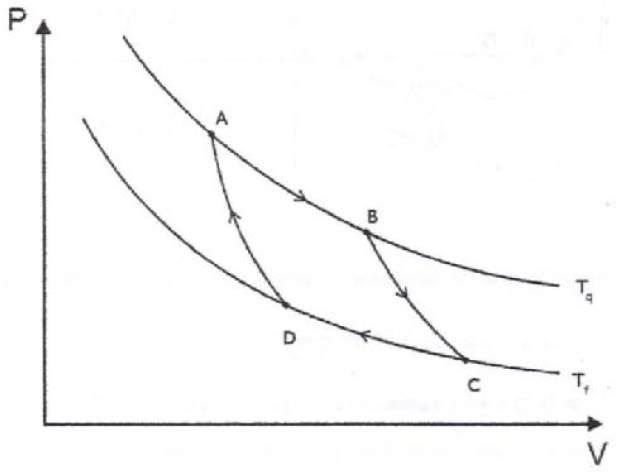
\includegraphics[scale=0.6]{termica-img/isoterma.png}
\end{figure}



\item Um mol de uma determinada substância percorre o ciclo formado pelos trechos $A \rightarrow B$, $B \rightarrow C$, $C \rightarrow D$ e $D \rightarrow A$ conforme mostrado no diagrama temperatura $T$ versus entropia $S$ da figura.
\begin{figure}[H]
  \centering
  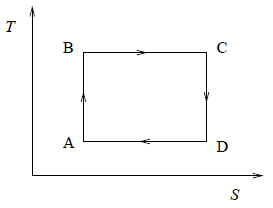
\includegraphics[scale=0.6]{termica-img/diagrama.png}
\end{figure}
São dados $TA$, $SA$ e as razões $\alpha = T_{B}/T_{A}$ e $r = S_{C}/S_{A}$. Determine em função dos dados do problema:

a) o calor trocado em cada um dos trechos e o trabalho total realizado no ciclo;
b) o rendimento $\eta$ de um motor que opera de acordo com esse ciclo;
c) o trabalho em cada um dos trechos do ciclo, considerando que a substância seja um gás ideal de capacidade térmica a volume constante $C_{V}$. Sugestão: utilize os resultados do item (a).
d) Esboce o ciclo no diagrama $P-V$ para a substância considerada no item anterior orientando e identificando o tipo de processo termodinâmico associado a cada um dos trechos.




\item Um corpo de capacidade térmica a pressão constante, $C_{P}$ (independente da temperatura), que se encontra inicialmente na temperatura $T_{1}$, é colocado em contato térmico com um reservatório térmico na temperatura $T_{2}$, sendo $x \equiv T_{1}/T_{2} < 1$. Após o equilíbrio térmico ter sido atingido, determine:

a) A variação da entropia do corpo.
b) A variação da entropia do reservatório.
c) A variação da entropia do Universo.
d) Verifique se o resultado obtido no item (c) está de acordo com a $2^{\underline{a}}$ lei da termodinâmica.



\item Um corpo de capacidade térmica $C$ constante é colocado em contato com um reservatório cuja temperatura $T_{0}$ se mantém invariante. Inicialmente, o corpo encontra-se à temperatura $T_{1}$ maior do que $T_{0}$. Determine a variação total de entropia $\Delta S$ e as variações da entropias do corpo e do reservatório. Indique se as variações são positivas ou negativas.


\item Mostre que
$$
\left( \frac{\partial T}{\partial p}  \right) = \frac{V}{C_{p}} (T\alpha - 1)
$$
onde $C_{p} = (\partial H/ \partial T)_{p}$ e $\alpha = (1/v) (\partial V/ \partial T)_{p}$


\item Determinar a energia média de $N$ osciladores independentes e de mesma frequência em contato com um reservatório térmico à temperatura $T$. A energia de cada oscilador é dada por
$$
E = \hbar \omega \left(  n + \frac{1}{2}  \right) \quad \quad n = 0,1,2,...
$$



\item Deduza a lei de Stefan-Boltzmann $u = \sigma T^{4}$ a partir da distribuição de Bose-Einstein. A densidade de estados para fótons é dada por
$$
g(\epsilon) = \frac{V}{\pi^{2}} \frac{\epsilon^{2}}{(c \hbar)^{3}}
$$
onde $\epsilon$ é a energia de um fóton e $V$ o volume. Determine a constante $\sigma$.




\item Considere um sistema de $N$ átomos localizados que não interagem entre si. Cada átomo pode estar em um de três estados diferentes. A energia de um dos estados é nula, enquanto os outros dois estados são degenerados, com energia $\Delta$. O sistema está em equilíbrio térmico a uma temperatura $T$.



a) Calcule a energia interna do sistema.

{\color{red}

O Hamiltoniano do sistema por ser escrito como:

$$
H=\sum_{j=1}^{N} \varepsilon_{j}
$$

onde $\epsilon_{j}$ é a energia do $j$-ésimo átomo. Como os átomos não interagem entre si, a função de
partição do sistema é

$$
Z = \operatorname{Tr}\left[e^{-\beta H}\right]=Z_{1}^{N}
$$

onde $Z_{1}$ é a função partição de um átomo e $\beta = (k_{B}T)^{-1}$. Esta última pode ser facilmente
calculada

$$
Z_{1}=1+2 e^{-\beta \Delta}
$$

donde se obtém

$$
Z=\left(1+2 e^{-\beta \Delta}\right)^{N}
$$

A energia interna pode agora ser calculada diretamente

$$
U=-\frac{\partial}{\partial \beta} \ln Z=N \frac{2 \Delta e^{-\beta \Delta}}{\left(1+2 e^{-\beta \Delta}\right)}
$$

}

b) Calcule a entropia do sistema.
{\color{red}

A energia livre de Helmholtz é:

$$
F=-k_{B} T \ln Z=-\frac{N}{\beta} \ln \left(1+2 e^{-\beta \Delta}\right)
$$

A entropia é dada por $S=k_{B} \beta^{2} \frac{\partial F}{\partial \beta}$, donde

$$
S=N k_{B} \ln \left(1+2 e^{-\beta \Delta}\right)+2 \Delta N k_{B} \beta \frac{e^{-\beta \Delta}}{\left(1+2 e^{-\beta \Delta}\right)}.
$$


}

c) Obtenha a entropia nos limites $T \rightarrow  0$ e $T \rightarrow \infty$ se $\Delta > 0$.

{\color{red}
Se $\Delta > 0$, então

(i) $T \rightarrow 0$, $\beta \rightarrow \infty$, $e^{-\beta \Delta} \rightarrow 0$, logo $S \rightarrow 0$

(ii) $T \rightarrow \infty$, $\beta \rightarrow \infty$, $e^{-\beta \Delta} \rightarrow 1$, assim $S \rightarrow k_{B} ln 3$.

}

d) Obtenha a entropia nos limites $T \rightarrow  0$ e $T \rightarrow \infty$ se $\Delta < 0$.


{\color{red}

Se $\Delta < 0$, então

(i) $T \rightarrow 0$, $\beta \rightarrow \infty$, $e^{-\beta \Delta} \rightarrow \infty$, logo $S \rightarrow N k_{B} \ln \left(2 e^{-\beta \Delta}\right)+\Delta N k_{B} \beta \rightarrow N k_{B} \ln 2$.

(ii) $T \rightarrow \infty$, $\beta \rightarrow 0$, $e^{-\beta \Delta} \rightarrow 1$, assim $S \rightarrow N k_{B} \ln 3$.

}

\item Um sistema de N íons magnéticos está em contato com um reservatório térmico a uma temperatura T. Seja $\sigma_{i}$, com $i = 1, 2, ..., N$, a variável que representa a projeção do spin do $i$-ésimo íon na direção z em unidade apropriadas. A variável $\sigma_{i}$ pode assumir os valores +1 ou -1. Considere que N seja um número par. O sistema é descrito pelo Hamiltoniano

$$
H = - J \sum_{k=1}^{N/2} \sigma_{2k-1} \sigma_{2k} - \mu_{B} h \sum_{i=1}^{N} \sigma_{i}.
$$

Segundo esse Hamiltoniano, cada íon possui momento magnético $\mu_{B}$ e está acoplado a um campo magnético externo h. Nele, vemos ainda que o primeiro íon só interage com o segundo, o terceiro só com o quarto, e assim sucessivamente, através de um acoplamento J.



  a) Calcule a função de partição para o caso N = 2, ou seja, para um único par de íons. \textit{Sugestão}: determine primeiramente as energias associadas a cada um dos microestados ($\sigma_{1}, \sigma_{2}$).

  \resposta

  b) Generalize sua resposta calculando agora a funão de partição para um sistema de N íons magnéticos. Ou seja, calcule a funão de partição para um sistema contendo $N/2$ pares de íons.

  \resposta

  c) Calcule o momento magnético total médio do sistema de $N$ íons em função dos parâmetros externos $h$ e $T$, e das constantes $J$ e $\mu_{B}$

  \resposta

  d) Qual o valor do momento magnético total médio no limite de $h \rightarrow 0$? Esse sistema pode representar um material ferromagnético? Justifique a sua resposta.

  \resposta



\item Um sistema de $N$ partículas distinguíveis não interagentes é descrito pelo hamiltoniano

\begin{equation}
  H = \sum_{i=1}^{N} \epsilon_{i}
\end{equation}

A energia de cada partícula $\epsilon_{i}$ só pode assumir dois valores: $\epsilon_{i} = 0$ ou $\epsilon_{i} = \Delta > 0$. Portanto, cada microestado do sistema é descrito pelo conjunto de valores ($\epsilon_{1}, \epsilon_{2},...,\epsilon_{N}$).


a) Se o sistema possui energia total $E$, que é um múltiplo inteiro de $\Delta$, o número total de microestados possíveis é
\begin{equation}
\Omega (E,N) = \frac{N!}{(E/\Delta)! (N - E/\Delta)!}
\end{equation}
Com base no postulado fundamental da mecênica estatística, qual é a probabilidade de se encontrar o sistema em um microestado específico?

\resposta O postulado estabelece que para energia fixa não há nenhum estado mais provável que outro (equiprobabilidade a priori), logo
$$
\operatorname{Pr}\left(\varepsilon_{1}, \varepsilon_{2}, \ldots, \varepsilon_{N}\right)=\frac{1}{\Omega(E, N)}=\frac{(E / \Delta) !(N-E / \Delta) !}{N !}
$$

b) Calcule a entropia por partícula do sistema $s = S/N$ como função da energia por partícula $u = E/N$ no regime $N>>1$. Utilize a aproximação $\operatorname{ln} N! \approx N \operatorname{ln}(N) - N$, válida para N>>1.

\resposta A entropia é dada por
$$
\begin{aligned}
S &=k_{B} \ln \Omega \\
&=k_{B} \ln N !-k_{B} \ln (E / \Delta) !-k_{B} \ln (N-E / \Delta) ! \\
& \approx k_{B} N \ln N-k_{B} N-k_{B}(E / \Delta) \ln (E / \Delta)+k_{B}(E / \Delta) \\
&-k_{B}(N-E / \Delta) \ln (N-E / \Delta)+k_{B}(N-E / \Delta)
\end{aligned}
$$
Dividindo por $N$ e reagrupando os termos,
$$
s=-k_{B} \frac{u}{\Delta} \ln \frac{u}{\Delta}-k_{B}\left(1-\frac{u}{\Delta}\right) \ln \left(1-\frac{u}{\Delta}\right)
$$

c) Determine a temperatura do sistema como função de $u$. Existe algum intervalo de valores de $u$ em  que a temperatura é negativa?

\resposta Como
$$
\frac{1}{T} = \frac{\partial s}{\partial u},
$$
obtemos
$$
T = \frac{1}{k_{B}} \frac{1}{\mathrm{ln} \left( \frac{\Delta - u}{u} \right)}.
$$
Nota-se que quando $\frac{\Delta - u}{u} < 1 \Rightarrow u > \Delta /2$, tem-se $T < 0$. O valor máximo de $u$ é $\Delta$. Assim, para $\Delta/2 < u \leq \Delta$, o sistema apresenta uma temperatura negativa. Isso é uma característica de sistemas cujo espectro de energias apresenta um valor máximo.


d) Calcule o calor específico do sistema. Existe algum regime em que o calor específico é negativo?

\resposta Da Eq. (11)
$$
u = \frac{\Delta}{1+e^{\Delta/k_{B}T}}
$$
O calor específico é dado por
$$
c=\frac{\partial u}{\partial T}=\frac{\Delta^{2} e^{\Delta /\left(k_{B} T\right)}}{k_{B} T^{2}\left(1+e^{\Delta /\left(k_{B} T\right)}\right)^{2}}
$$
Desta expressão, vê-se claramente que $c \geq 0$, ou seja, o calor específico nunca é negativo.





\item Considere um gás de $N >> 1$ partículas pontuais \textbf{clássicas} de massa $m$ em uma caixa cúbica ($0 \leq x \leq L$, $0 \leq y \leq L$, $0 \leq z \leq L$) nas proximidades da superfície da Terra. As partículas estão sujeitas aos potencial gravitacional $V(z) = mgz$, onde $g$ é a aceleração gravitaciona e $z$ é a altura da partícula em relação à superfície da Terra. O gás encontra-se em equilíbrio à temperatura $T$.



  a) Escreva a hamiltoniana de uma única partícula na caixa como função de suas coordenadas e das componentes do momento linear $p_{x}$, $p_{y}$ e $p_{z}$.

  \resposta

  b) Encontre a função de partição do sistema de $N$ partículas \textbf{clássicas}.

  \resposta

  c) Suponha que $mgL << k_{B}T$ e encontre a funão de partição nesse regime. Você pode usar a seguinte aproximação: $e^{-x} \approx 1 - x$, se $x << 1$.

  \resposta

  d) Obtenha a pressão dos gás no regime do item (c) em função de $N$, $T$ e $V = L^{3}$.

  \resposta



\item Considere um sistema formado por $N$ átomos localizados e independentes. Cada átomo tem quatro estados quânticos possíveis: o primeiro estado tem energia 0, o segundo e terceiro estados são degenerados com energia $2\epsilon$ e o quarto e último estado tem energia $3\epsilon$ ($\epsilon > 0$). O sistema encontra-se em equilíbrio à temperatura $T$.


a) Calcule a energia livre de Helmholtz do sistema.

\resposta

b) Calcule a energia interna por partícula do sistema.

\resposta

c) Calcule a entropia do sistema.

\resposta

d) Obtenha a entropia por partícula do sistema nos limites $T \rightarrow 0$ e $T \rightarrow \infty$. Interprete fisicamente os resultados.

\resposta




\item Um sistema de $N$ osciladores quânticos unidimensionais, localizados e independentes está em equilíbrio com um reservatório térmico à temperatura $T$. As energias de cada oscilador são dadas por

$$
E_{n} = \hbar \omega_{0} \left(  n + \frac{1}{2} \right)   \quad \quad n = 1,3,5,7,...
$$


\textbf{Note que os valores assumidos por $n$ são apenas os naturais ímpares.}


a) Obtenha uma expressão para a energia interna por oscilador $u$ como função da temperatura $T$. Qual é a expressão para $u$ no limite clássico ($\hbar \omega_{0} << k_{B}T$)? Esboce um gráfico de $u$ por $T$.

\resposta (a) Podemos escrever
$$
E_{n}=\hbar \omega_{0}\left(2 n+1+\frac{1}{2}\right)=\hbar \omega_{0}\left(2 n+\frac{3}{2}\right) \quad n=0,1,2, \ldots
$$
I função de partição para o ensemble canônico de um oscilador é
$$
Z_{1}=\sum_{n=0}^{\infty} e^{-\beta \hbar \omega_{0}\left(2 n+\frac{3}{2}\right)}=e^{-\frac{3}{2} \beta \hbar \omega_{0}} \sum_{n=0}^{\infty} e^{-2 \beta \hbar \omega_{0} n}=e^{-\frac{3}{2} \beta \hbar \omega_{0}} \sum_{n=0}^{\infty} x^{n}
$$
ende $\beta \equiv \frac{1}{k_{B} T}$ e $x=e^{-2 \beta \hbar \omega_{0}} .$ Usando $\sum_{n=0}^{\infty} x^{n}=1 /(1-x)$
$$
Z_{1}=\frac{e^{-\frac{3}{2} \beta \hbar \omega_{0}}}{1-e^{-2 \beta \hbar \omega_{0}}}
$$
I função de partição para o sistema de $N$ osciladores $é Z=Z_{1}^{N} .$ A energia interna por oscilador
$$
\begin{aligned}
u &=\frac{U}{N}=-\frac{1}{N} \frac{\partial}{\partial \beta} \ln Z=-\frac{\partial}{\partial \beta} \ln Z_{1}=\frac{\partial}{\partial \beta}\left[\frac{3}{2} \beta \hbar \omega_{0}+\ln \left(1-e^{-2 \beta \ln \omega_{0}}\right)\right] \\
&=\frac{3}{2} \hbar \omega_{0}+\frac{2 \hbar \omega_{0} e^{-2 \beta \hbar \omega_{0}}}{1-e^{-2 \beta \hbar \omega_{0}}}=\hbar \omega_{0}\left(\frac{3}{2}+\frac{2}{e^{2 \beta \hbar \omega_{0}}-1}\right)
\end{aligned}
$$
To limite clássico $\hbar \omega_{0} \ll k_{B} T, e^{2 \beta \text { hwo }} \approx 1+2 \beta \hbar \omega_{0}$ e
$$
u \approx \hbar \omega_{0}\left(\frac{3}{2}+\frac{2}{2 \beta \hbar \omega_{0}}\right)=\frac{3}{2} \hbar \omega_{0}+k_{B} T \approx k_{B} T
$$
\begin{figure}[H]
  \centering
  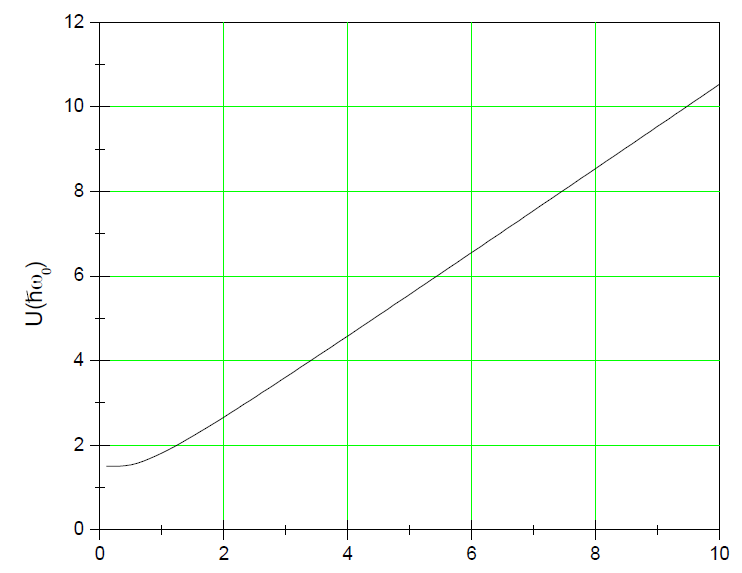
\includegraphics[scale=0.6]{termica-img/osciladores.png}
  \caption{Esboço de $u \times T$}
\end{figure}



b) Obtenha uma expressão para a entropia por oscilador $s$ como função da temperatura $T$. Qual é a expressão para $s$ no limite clássico? Esboce um gráfico de $s$ por $T$.

\resposta A entropia por oscilador é
$$
\begin{aligned}
s &=\frac{S}{N}=\frac{U-F}{N T}=\frac{u}{T}+\frac{k_{B} \ln Z}{N}=\frac{u}{T}+k_{B} \ln Z_{1} \\
&=\frac{\hbar \omega_{0}}{T}\left(\frac{3}{2}+\frac{2}{e^{2 \beta h \omega_{0}}-1}\right)-k_{B}\left[\frac{3}{2} \beta \hbar \omega_{0}+\ln \left(1-e^{-2 \beta h \omega_{0}}\right)\right] \\
&=\frac{2 \hbar \omega_{0} / T}{e^{2 \beta h \omega_{0}}-1}-k_{B} \ln \left(1-e^{-2 \beta \hbar \omega_{0}}\right)
\end{aligned}
$$
onde usamos alguns resultados do item (a). No limite clássico
$$
s \approx \frac{2 \hbar \omega_{0} / T}{2 \beta \hbar \omega_{0}}-k_{B} \ln \left(2 \beta \hbar \omega_{0}\right)=k_{B}\left[1+\ln \left(\frac{k_{B} T}{2 \hbar \omega_{0}}\right)\right]
$$
\begin{figure}[H]
  \centering
  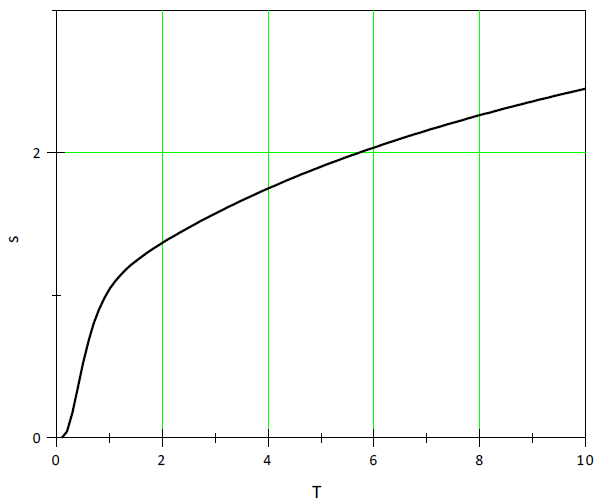
\includegraphics[scale=0.6]{termica-img/osciladores1.png}
  \caption{Esboço de $s \times T$}
\end{figure}






\item Considere um sistema formado por N íons magnéticos localizados de spin 1 em contato com um reservatório térmico à temperatura $T$. O sistema é descrito de forma simplificada pelo Hamiltoniano

$$
H = D \sum_{i=1}^{N} \sigma_{i}^{2} - h \sum_{i=1}^{N} \sigma_{i},
$$

onde $\sigma_{i}$ é a projeção $z$ (adimensional) do spin $i$, que pode assumir os valores 0, $+1$ e $-1$, $h > 0$ é um campo magnético externo e $D > 0$ é um termo de anisotropia.


a) Determine a função de partição do sistema.
b) Determine a energia livre de Helmholtz por íon como função da temperatura.
c) Determine a energia interna por íon como função da temperatura.
d) Suponha agora que $h = 0$. Determine o calor específico como função da temperatura.



\item Considere um sistema de $N$ spins $1/2$ não-interagentes, com momento de dipolo magnético de módulo $\mu$, na presença de um campo magnético uniforme $B$.


a) Escreva a hamiltoniana do sistema.
b) Considerando o sistema em equilíbrio térmico a temperatura inversa $\beta = 1/k_{B}T$, calcule a função de partição $Z(\beta;B)$.
c) Calcule a magnetização $M$ como função de $T$ e $B$.
d) Obtenha a expressão para $M$ no limite de altas temperaturas e campo magnético fraco.



\item Num modelo para um cristal sólido podemos supor que os $N$ átomos sejam equivalentes a $3N$ osciladores harmônicos clássicos, unidimensionais, independentes, de massa $m$, que oscilam com a mesma frequência angular $\omega$ em torno de sua posição de equilíbrio. A uma distância $x$ desta posição a energia potencial é dada por $U = m\omega^{2}x^{2}/2$. Conhecendo-se alguns dados experimentais, é possível estimar, em termos da distância inter-atômica a baixas temperaturas $d$, a raiz do deslocamento quadrático médio dos átomos quando ocorre a fusão. A resolução dos itens abaixo permite fazer esta estimativa. Suponha que o sólido se encontre em equilíbrio térmico a uma temperatura absoluta $T$.


a) Considere que o número de estados numa célula do espaço de fase ($x, p$) seja dado por $(dxdp)/h$, onde $h$ é a constante de Planck. Obtenha a função de partição para o oscilador harmônico, $Z(T,\omega)$.

\resposta A função de partição é obtida somando sobre todos os estados do sistema com o peso de Boltzmann
%
\begin{equation}
  Z = Tr e^{-\beta H} = \int_{-\infty}^{\infty} \int_{-\infty}^{\infty} \frac{dx dp}{h} exp \left[ - \beta \left( \frac{p^{2}}{2m} + \frac{m \omega^{2} x^{2} }{2}  \right)  \right] ,
\end{equation}
%
onde $\beta^{-1} = k_{B} T$. Usando
%
\begin{equation}
  \int_{-\infty}^{\infty} dx e^{-\alpha x^{2}} = \sqrt{\frac{\pi}{a}} ,
\end{equation}
%
obtemos
%
\begin{equation}
  Z = \frac{\pi}{h} \sqrt{ \frac{2m}{\beta} } \sqrt{\frac{2}{\beta m \omega^{2}}}
\end{equation}
%
\begin{equation}
  Z = \frac{2 \pi k_{B} T}{h \omega} = \frac{k_{B} T}{\hbar \omega} .
\end{equation}



b) Calcule o número médio de osciladores cuja posição se encontra entre $x$ e $x + dx$.

\resposta Como os osciladores são independentes, o número médio $n(x)dx$ pedido é igual a $3N$ vezes a probabilidade de um oscilador ter sua posição no intervalo considerado. Esta probabilidade, por sua vez, é igual ao peso de Boltzmann integrado sobre todos os valores de momento linear, donde
%
\begin{equation}
  n(x) dx = \frac{3N dx}{Z} \int_{-\infty}^{\infty} \frac{dp}{h} exp \left[ - \beta \left( \frac{p^{2}}{2m} + \frac{m \omega^{2} x^{2}}{2} \right) \right]
\end{equation}
%
\begin{equation}
  n(x) dx = 3N\omega dx  \sqrt{\frac{m}{2 \pi k_{B} T}}   exp \left( - \frac{ m \omega^{2} x^{2} }{2 k_{B} T} \right) .
\end{equation}


c) Obtenha uma expressão para a energia potencial média, $\langle U\rangle$ por oscilador unidimensional. Compare o resultado com o valor esperado pelo teorema da equipartição.

\resposta A energia potencial média por oscilador é
%
\begin{equation}
\begin{array}{ccc}
  \langle U \rangle &=& \frac{1}{3N} \int_{-\infty}^{\infty} \left( \frac{ m \omega^{2} x^{2} }{2}  \right) n(x)dx \\
   & = & \omega \sqrt{\frac{m}{2 \pi k_{B} T}} \int_{-\infty}^{\infty} \left( \frac{m \omega^{2} x^{2}}{2} \right) exp \left( - \frac{ m \omega^{2} x^{2} }{2 k_{B} T} \right) dx \\
    & = & \omega \sqrt{\frac{m}{2 \pi k_{B} T}} (k_{B} T)  \sqrt{\frac{2 k_{B} T}{m \omega^{2}}} \int_{-\infty}^{\infty} x^{2} e^{-x^{2}} dx .
\end{array}
\end{equation}
%
Usando que $\int_{-\infty}^{\infty} x^{2} e^{-x^{2}} = \sqrt{\pi} / 2 $,
%
\begin{equation}
 \langle U \rangle = \frac{k_{B} T}{2} .
\end{equation}
%
Esse resultado é o esperado pelo teorema da equipartição, que diz que o valor médio clássico de cada grau de liberdade quadrático da Hamiltoniana (como a energia potencial) é $k_{B}T/2$.


d) Seja $x_{0}^{2}$ o deslocamento quadrático médio em torno do equilíbrio quando o sólido se funde e seja $f = x_{0}/d$. Usando $\langle U\rangle = m\omega^{2}x_{0}^{2}/2$, estime $f$ para um dado elemento cuja massa atômica é $m = 1.0 \times 10^{-25} \ kg$, a temperatura de fusão é $T_{F} = 1400 \ K$, $d = (10/3) \ \AA = (10/3)\times 10^{-10} \ m$ e a frequência é tal que $\hbar \omega/k_{B} = 300 \ K.$

\resposta Temos que
%
\begin{equation}
  \frac{m \omega^{2} x_{o}^{2} }{2} = \frac{k_{B} T}{2} \ \ \Rightarrow \ \ f = \frac{x_{o}}{d} = \frac{1}{\omega d} \sqrt{\frac{k_{B}T}{m}} .
\end{equation}
%
Para os dados fornecidos
%
$$
f \approx 0.03 = 3 \%
$$






\item Considere $N$ osciladores harmônicos tridimensionais clássicos não-interagentes, de massa $m$ e frequência angular $\omega$, em contato com um reservatório térmico à temperatura $T$.


a) Escreva a hamiltoniana do sistema e obtenha a função de partição canônica.
b) Obtenha o valor médio da energia por oscilador. Qual a capacidade térmica do sistema?





\item Considere um sistema composto por um número grande $N$ de moléculas distinguíveis, que não interagem entre si. Cada molécula tem dois estados de energia possíveis: 0 e $\epsilon > 0$.


a) Obtenha a densidade de entropia S/N do sistema como função apenas da energia média por molécula E/N, de $\epsilon$ e da constante de Boltzmann $k_{B}$.
b) Considerando o sistema em equilíbrio térmico à temperatura inversa $\beta = 1 / k_{B}T$, calcule $E/N$.
c) Qual o valor máximo para $E/N$ no caso acima? Compare com o valor máximo dessa grandeza caso fosse possível que todos os elementos do sistema estivessem no estado de energia máxima.




\item Um determinado material magnético é composto por $N$ átomos magnéticos não-interagentes, cujos momentos magnéticos $\mu$ podem apontar em três direções possíveis, conforme mostra a figura ao lado: $\boldsymbol{\mu}_{0} = \mu \hat{\boldsymbol{y}}$, $\boldsymbol{\mu}_{1} = \mu \hat{\boldsymbol{x}}$ e $\boldsymbol{\mu}_{2} = - \mu \hat{\boldsymbol{x}}$. O sistema encontra-se em equilíbrio térmico a temperatura $T$ e na presença de um campo magnético uniforme orientado ao longo da direção $y$, $\boldsymbol{H} = H \hat{\boldsymbol{y}}$, de modo que os níveis de energia correspondentes a um único átomo são $\epsilon_{0}= -\mu H$, $\epsilon_{1}= 0$ e $\epsilon_{2}= 0$.

\begin{figure}[H]
  \centering
  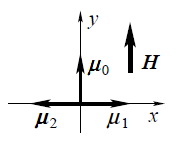
\includegraphics[scale=0.8]{termica-img/momento.png}
\end{figure}


a) Obtenha a função de partição canônica $z$ de um átomo, a função de partição canônica $Z$ do sistema e a energia livre de Helmholtz $f$ por átomo.
b) Determine a energia média $u = \langle \epsilon_{n} \rangle$ e a entropia $s$ por átomo.
c) Obtenha a magnetização por átomo $\mathbf{m} = m_{x}\hat{x} + m_{y} \hat{y} = \langle \boldsymbol{\mu}_{n} \rangle$.
d) Verifique que a susceptibilidade isotérmica $\chi_{T} = (\partial m_{y} / \partial H)_{T}$ a campo nulo obedece à lei de Curie, $\chi_{T}  \propto 1/T$.





\item Considere um gás monoatômico clássico constituído por $N$ átomos não interagentes de massa $m$ confinados num recipiente de volume $V$ , à temperatura $T$. A hamiltoniana corespondente a um átomo é dada por $\mathcal{H} = \left( p_{x}^{2} + p_{y}^{2} + p_{z}^{2} \right) / 2m$.


  a) Mostre que a função de partição canônica atômica é  $\zeta=V / \lambda^{3}$, onde $\lambda=h / \sqrt{2 \pi m k_{B} T}$ o comprimento de onda térmico de de Broglie.
  b) Utilizando $\zeta$ do item anterior, obtenha a função de partição $Z$ do sistema e a energia livre de Helmholtz $F$. Obtenha, também, a energia livre por átomo $f = F/N$ no limite termodinâmico $N \rightarrow \infty$, $V \rightarrow \infty$, $v = V/N$ fixo.
  c) Obtenha a energia interna $U$ e a pressão $p$ do gás.
  d) Calcule a entropia por átomo no limite termodinâmico.




\item A radiação em uma cavidade ressonante pode ser vista como um gás de fótons cuja pressão sobre as paredes de uma cavidade de volume $V$ é dada por
$$
P = \frac{\alpha T^{4}}{3}
$$
onde $a$ é uma constante. A energia interna desse gás é dada pela equação $U = \alpha T^{4} V$. Considere que inicialmente a temperatura da cavidade seja $T_{0}$ e seu volume $V_{0}$.


a) Determine o trabalho realizado em um processo isotérmico no qual o volume da cavidade é duplicado. Forneça a resposta em termos de $T_{0}$, $V_{0}$ e da constante $a$ apenas.
b) Determine o calor fornecido em um processo isotérmico no qual o volume da cavidade é duplicado. Forneça a resposta em termos de $T_{0}$, $V_{0}$ e da constante $a$ apenas.
c) Usando a relação
$$
\mathrm{d} Q=\left(\frac{\partial U}{\partial T}\right)_{V} d T+\left[\left(\frac{\partial U}{\partial V}\right)_{T}+P\right] d V
$$
determine a equação que descreve um processo adiabático em termos das variáveis $V$ e $T$.
d) Determine o trabalho realizado em um processo adiabático no qual o volume da cavidade é duplicado. Expresse o resultado em termos de $T_{0}$, $V_{0}$ e da constante $a$ apenas.




\item Considere um oscilador harmônico unidimensional modificado, definido pela função hamiltoniana
$$
\mathscr{H}=\frac{p^{2}}{2 m}+V(x)
$$
onde $V(x)=\frac{1}{2} m \omega^{2} x^{2}$ para $x \geq 0$, $V(x)=\infty$  para $x<0$. Ele encontra-se em equilíbrio térmico com um reservatório de calor a temperatura $T$.


a) Justifique, em termos da paridade das autofunções do problema quântico, por que, devido às condições impostas, apenas os valores inteiros ímpares de $n$ são permitidos para as autoenergias deste oscilador, $\epsilon_{n} = (n + 1/2)\hbar \omega$.
b) Para a versão quântica, obtenha a funçãao de partição canônica $z$ deste oscilador e a energia livre de Helmholtz associada $f$.
c) Obtenha a energia interna média deste oscilador a partir de $u = -\partial \operatorname{ln} z/ \partial \beta$.
d) A partir da definição da energia interna média no ensemble canônico, $u \equiv \langle \epsilon_{n} \rangle$, demonstre a expressão $u = -\partial \operatorname{ln}z / \partial \beta$.
e) Mostre que a função de partição canônica clássica deste oscilador é dada por $z_{class} = (2\beta \hbar \omega)^{-1}$. Determine a energia interna média clássica associada, $u_{class} \equiv \langle \mathscr{H} \rangle_{class}$.




\item Considere um mol ($n = 1$) de um gás ideal monoatômico, inicialmente no estado de equilíbrio térmico especificado pela pressão $P_{0}$ e pelo volume $V_{0}$. Esse gás sofre uma compressão adiabática reversível que o leva a ocupar um volume $V_{0}/2$. Determine:


a) a variação de energia interna desse gás devido a essa compressão;
b) a variação de entropia do gás nessa compressão.

Após essa compressão adiabática, o gás, sempre isolado do resto do universo por paredes adiabáticas, sofre uma expansão completamente livre até o volume original $V_{0}$. Determine:

c) a variação de temperatura do gás devido à expansão livre;
d) a variação de entropia do gás nessa expansão livre.





\item Considere um gás composto por $N$ partículas ultrarrelativísticas (de forma que sua energia $\epsilon$ possa ser escrita como $\epsilon = cp$ , onde $p$ é o seu momento linear) confinado em um recipiente de volume $V$ e a temperatura $T$. Suponha que as partículas sejam indistinguíveis e não interagentes, e que sua energia térmica seja suficientemente alta para desprezar efeitos quânticos.

a) Mostre que a função de partição do gás é $Z=\frac{(8 \pi V)^{N}}{N !\left(h c / k_{B} T\right)^{3 N}}$, onde $h$ é a constante de Planck, c é a velocidade da luz no vácuo e $k_{B}$ é a constante de Boltzmann.
b) Determine a pressão do gás.
c) Calcule a entropia do gás.
d) Determine a energia interna do gás.





\item Imagine que um material magnético unidimensional possa ser modelado como uma cadeia linear de $N + 1$ spins. Cada spin interage com os seus primeiros vizinhos de tal maneira que a energia do sistema seja $E = n^{2} \epsilon$, onde $n$ é o número de paredes de domínio separando regiões de spin $\shortuparrow$ das regiões de spin $\shortdownarrow$, como representado na figura abaixo, sendo as paredes de domínio indicadas por linhas tracejadas. A energia por parede de domínio é $\epsilon$. Considere $N >> 1$ e $n >> 1$.

a) Determine de quantas maneiras as $n$ paredes de domínio podem ser arranjadas.
b) Determine a entropia $S(E)$ do sistema contendo $n$ paredes de domínio.
c) Determine a energia interna $E$ como função da temperatura, $E(T)$. Expresse seu resultado em termos de $N$, $\epsilon$, $T$ e constantes físicas apenas.
d) Esboce a função $E(T)$, indicando os valores de $E$ para $T = 0$ e $T \rightarrow \infty$.

\begin{figure}[H]
  \centering
  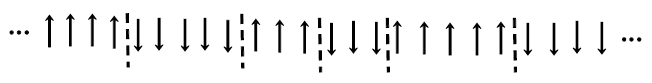
\includegraphics[scale=0.8]{termica-img/spin.png}
\end{figure}



\item Um mol de um gás ideal monoatômico se encontra na temperatura $T$ e ocupa um volume $V$. A energia interna por mol de um gás ideal é dada por $u = c_{V} T$, onde $c_{V}$ é o calor específico molar, que é considerado constante. Responda as questões abaixo:

a) Considere a situação em que o gás se encontra em contato com um reservatório térmico na temperatura $T$ e sofre uma expansão quase-estática reversível na qual o seu volume passa de $V$ para $2V$ . Calcule o trabalho realizado pelo gás durante a sua expansão.
b) Ainda com relação ao processo físico descrito no item (a), determine o calor trocado pelo gás com o reservatório térmico.
c) Determine as variações de entropia do gás e do reservatório térmico no processo descrito no item (a).
d) Considere agora a situação em que o gás está isolado e sofre uma expansão livre na qual o seu volume passa de $V$ para $2V$. Determine as variações de entropia do gás e do universo durante o processo de expansão livre.




\item A lei de Stefan-Boltzmann diz que a densidade de energia total do campo eletromagnético dentro de uma cavidade em equilíbrio térmico é dada por
$$
u(T) = a T^{4},
$$
onde $a$ é uma constante.


  a) Podemos derivar a lei de Stefan-Boltzmann usando argumentos termodinâmicos. Sabendo que, em equilíbrio termodinâmico, a densidade de energia da radiação independe do material que forma as paredes, podemos concluir que qualquer variável extensiva da radiação em uma cavidade deverá ser proporcional ao volume da cavidade e depender apenas da temperatura. Em particular, a energia interna e a entropia da radiação serão $U = u(T) V$ e $S = s(T) V$, respectivamente. Podemos usar o eletromagnetismo clássico para calcular a pressão de radiação nas paredes da cavidade. Ela tem a forma de $P = \frac{u(T)}{3}$. Usando essas informações e a primeira lei da termodinâmica, demonstre a lei de Stefan-Boltzmann.
  b) Agora obtenha esse resultado usando física estatística, assumindo que a radiação eletromagnética é um gás de fótons.
  
    \item[i.] Calcule a função de partição, $Z$, e mostre que o número médio de fótons com energia $\epsilon_{j}$ é
    $$
    \overline{n}_{f} = - \frac{1}{\beta} \frac{\partial \operatorname{ln} Z}{\partial \epsilon_{j}} = \frac{1}{e^{\beta \epsilon_{j} - 1}},
    $$
    onde $\beta = \frac{1}{k_{\beta}T}$.
    \item[ii.] Obtenha a lei de Stefan-Boltzmann. Você pode usar que o número total de fótons por unidade de volume e frequência entre $[\omega, \omega + d \omega]$ é dado por
        $$
        g(\omega)d\omega = k \frac{\omega^{2} d \omega}{e^{\beta \epsilon_{\omega}} - 1},
        $$
        onde $k$ é uma constante e $\epsilon_{\omega} = \hbar \omega$ é a energia de um fóton.
  






\item Um gás ideal de moléculas diatômicas polares, cada uma com momento de dipolo elétrico $\vec{\mu}$, encontra-se a uma temperatura $T$ e está sujeito a um campo elétrico $\vec{\varepsilon}$. As orientações dos dipolos são definidas pelos ângulos $\theta(0 \leq \theta \leq \pi)$ e $\phi ( 0 \leq \phi \leq 2 \pi)$ de um sistema de coordenadas esféricas cujo eixo$-z$ é paralelo ao campo elétrico. A probabilidade de encontrar uma molécula com orientação do dipolo dentro do elemento $d\theta d\phi$ vale $\rho d \theta d \phi$ onde $a$ densidade de probabilidade $\rho(\theta, \phi)$ é dada por
$$
\rho (\theta, \phi) = \frac{1}{A} \operatorname{sen} \theta e^{-\beta E},
$$
e está normalizada de acordo com $\int \rho(\theta, \phi)d\theta d \phi = 1$. A constante $A$ é um fator de normalização, $\beta = 1/k_{B} T$, $k_{B}$ é a constante de Boltzmann e $E$ é a energia de interação do momento de dipolo com o campo, dada por $E = - \vec{\mu} \cdot \vec{ \varepsilon} = - \mu \varepsilon \operatorname{cos} \theta$.

a) Determine $A$ como função de $T$, $\varepsilon$ e $\mu$.
b) O momento de dipolo médio por molécula é definido pela média $P = \mu \langle \operatorname{cos} \theta \rangle$. Determinar $P$ como função de $T$ e $\varepsilon$.
c) Esboce o gráfico de $P$ versus $\varepsilon$ para $T$ constante.
d) A susceptibilidade elétrica é definida por $\chi = \partial P / \partial \varepsilon$. Determine $\chi$ a campo nulo e mostre que ela é inversamente proporcional à temperatura $T$. Notar que para pequenos valores de $x$ vale $\operatorname{coth} x \approx 1/x + x/3$.



\item A função de partição de um gás monoatômico de $N$ partículas interagentes pode ser escrita como:
$$
Z = \left(  \frac{N - Nb}{N}  \right)^{N} \left(  \frac{mk_{B}T}{2\pi \hbar^{2}}  \right)^{\frac{3N}{2}} exp \left(  \frac{N^{2} a}{V k_{B} T}  \right),
$$
onde $a$ e $b$ são constantes positivas e $m$ a massa da partícula.

a) Determine a energia livre de Helmholtz do gás.
b) Determine a equação de estado desse gás, em termos da pressão, do volume específico $v = V/N$, da temperatura e de constantes.
c) Determine a energia interna específica $u = U/N$ do gás.
d) Considere que o gás sofra um processo de expansão livre no qual seu volume inicial $V$ é duplicado no interior de um recipiente feito de paredes adiabáticas. Calcule a variação da temperatura absoluta que ocorre no processo.



\item (a) Dadas as equações de estado empíricas para um gás ideal,
$$
p = \frac{RT}{v} \quad \quad u = \frac{3}{2} RT
$$
onde $v$ e $u$ são, respectivamente, volume molar e energia molar, mostre, a partir da primeira lei da Termodinâmica, que a sua função entropia molar é dada por $s(u, v) = R \operatorname{ln} (u^{3/2} v) + s_{0}$. Deduza a mesma função, $s(u,v)$, a partir do cálculo da função de partição no ensemble canônico.


  b) Um mol de gás monoatômico, contido em recipiente de volume $V$, a uma temperatura $T$, efetua uma expansão livre para um volume $2V$. A expansão livre ocorre com isolamento térmico.
      
        \item[i.] Obtenha a variação de energia interna e de entropia. Justifique.
        \item[ii.] Represente esquematicamente um gráfico de entropia como função do volume e identifique nele os estados inicial e final do gás. Explique a variação de entropia com o volume, utilizando a interpretação microscópica para a entropia.
        \item[iii.] Qual é a variação da pressão, na expansão livre? Verifique se a representação gráfica do ítem anterior está de acordo com esta variação.
      



\item Os cosmologistas consideram o universo como uma cavidade eletromagnética em expansão isentrópica contendo radiação a uma temperatura de $2,7 K$.

  a) Use a equação de Gibbs-Duhem para a entropia para provar que a pressão da radiação é dada por $p = \frac{U}{3V}$, onde $U$ é a energia e $V$ é o volume da cavidade.
  b) Qual será a temperatura desta radiação, se o volume dobrar?
  c) Bartoli (1876) utilizou a $2^{\underline{a}}$ lei da Termodinâmica para provar a necessidade da existência de uma pressão da radiação eletromagnética (que não era óbvia, antes do final do século XIX!), numa demonstração utilizada posteriormente por Boltzmann. A prova baseia-se na seguinte situação: um recipiente de paredes perfeitamente refletoras tem três compartimentos internos separados também perfeitamente refletoras nas duas faces (veja figura 2). A radiação contida nos compartimentos 1 e 2 estão inicialmente a uma mesma temperatura $T_{1} = T_{2}$, menor do que a temperatura da radiação contida no compartimento 3, $T_{3}$. Faz-se um furo na parede B e simultaneamente desloca-se a parede A em direção à parede B, até que as duas se encontrem. Dessa maneira, transfere-se energia do compartimento 2 (mais frio) para o compartimento 3 (mais quente). Explique claramente porque a $2^{\underline{a}}$ lei deixa de ser violada se existir uma pressão da energia eletromagnética.
      \begin{figure}[H]
  \centering
  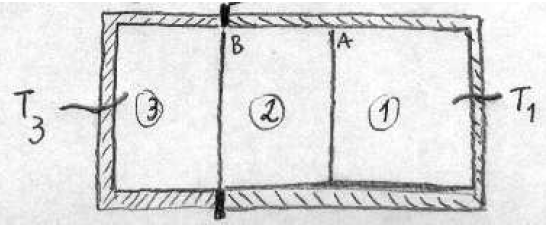
\includegraphics[scale=0.8]{termica-img/pressaoradiacao.png}
\end{figure}



\item No enunciado do princípio de conservação de energia, Mayer usou o fato, já conhecido na época, de que o calor específico a pressão constante é maior do que o calor específico a volume constante.

  a) Discuta a aplicação do princípio geral de conservação de energia no contexto da Termodinâmica.
  b) Justifique fisicamente porque o calor específico a pressão constante é maior do que o calor específico a volume constante.



\item Boltzmann propõe descrever a função termodinâmica entropia, para um sistema isolado, como $S = k \operatorname{ln} W$, onde $W$ é o número de estados acessíveis ao sistema.

  a) Qual é a hipótese estatística associada a esta expressão para a entropia?
  b) Explique fisicamente a relação entre os ensembles microcanônico e canônico. Exemplifique, utilizando um sistema pequeno (um "sólido" de duas partículas, com dois estados não degenerados cada uma, por exemplo).
  c) Esquematize um gráfico de distribuição de probabilidades em função da energia, para os estados do sistema pequeno, no ensemble canônico. Justifique.



\item A estatística clássica de Maxwell-Boltzmann pode ser aplicada aos gases ideais sob a condição de que o comprimento de onda térmico obedeça a seguinte relação: $\lambda^{3} << V/N$, onde $\lambda \equiv  \left( 3mk_{B} T / h^{2} \right)^{-1/2}$, $m$ é a massa da partícula de gás, $T$ é a temperatura, $V$ é o volume e $N$ é o número de partículas.

  a) Essa relação pode ser deduzida com argumentos semi-quantitativos utilizando-se a equipartição de energia e a descrição de estados quantizados de partículas livres em uma caixa. Utilize estes argumentos para justificá-la.
  b) Quais fatores você acha que contribuem para que o gás de elétrons no metal exija um tratamento de estatística quântica (Fermi-Dirac), ao passo que o gás de moléculas permite um tratamento com estatística clássica (Maxwell-Boltzmann)? Explique.
  \item[] (Dados: densidade do metal $\simeq 3 \times 10^{28}$ átomos$/m^{3}$, densidade do gás $\simeq 3 \times 10^{25}$ átomos$/m^{3}$).





\item Considere um sistema composto por um gás ideal monoatômico bidimensional, de $N$ átomos, contido em uma superfície de área $L^{2}$. O sistema encontra-se a uma temperatura T.

  a) Escreva a função de partição deste sistema e, a partir dela, encontre sua energia média. Este era o resultado que você esperava? Comente.
  b) Se as moléculas interagissem entre si através de um potencial $U(r_{1}, r_{2},...r_{N})$, discuta o que se modificaria na expressão da função de partição. Que modificação você esperaria ter na expressão da energia média?



\item Considere a expansão livre de um gás ideal (ou seja: um mol de gás está contido em uma das partições de um recipiente rígida, de paredes isolantes, dividido em duas partes iguais, e um furo na parede interna permite que o gás se expanda).

  a) Descreva qualitativamente o processo, do ponto de vista da energia e da entropia do gás. Justifique claramente suas resposta.
  b) Qual o comportamento da energia livre do gás durante o processo de expansão se o recipiente tiver paredes diatérmicas e estiver imerso em banho térmico? Justifique e relacione sua resposta com a $2^{\underline{a}}$ lei da termodinâmica.




\item Considere um ciclo de um gás que consiste de três transformações, na seguinte sequência: (i) 1-2 expansão isotérmica, (ii) 2-3 isobárica e (iii) 3-1 isovolumétrica.

  a) Represente o ciclo em um diagrama $p-V$ e, sem fazer contas, coloque as temperaturas e energias internas dos três estados em ordem crescente, supondo que a substância de trabalho é um gás de Van der Waals (as partículas interagem por mio de um potencial atrativo de longo alcance e repulsivo de curto alcance). Justifique.
  b) A relação fundamental para entropia por mol do gás de Van der Waals é dada por $s(u,v) = R \operatorname{ln} \left[ \left(v - b \right) \left( u + \frac{a}{v} \right)^{\frac{3}{2}} \right]$. Obtenha as expressões para a energia interna e a pressão, como funções da temperatura e do volume, respectivamente $u(T,v)$ e $p(T,v)$. Verifique se suas respostas ao ítem anterior, quanto aos processos 1-2 e 3-1, estão corretas.




\item Considere um sistema de duas partículas idênticas não interagentes, $X$ e $Y$, as quais possuem dois estados de partícula, 1 e 2, de energias respectivas $\epsilon_{1}$ e $\epsilon_{2}$.

  a) Especifique os estados deste sistema para os três casos: i) bósons, ii) férmios e iii) partículas clássicas.
  b) Escreva a função de partição canônica do sistema para os três casos, $Z_{B}$, $Z_{F}$ e $Z_{Ct}$, respectivamente. Comente as probabilidades dos diversos estados.





\item Considere o ciclo de Carnot, composto de duas etapas isotérmicas, $1 \rightarrow 2$ e $3 \rightarrow 4$, e duas adiabáticas, $2 \rightarrow 3$ e $4 \rightarrow 1$.

a) O ciclo de Carnot, se realizável, seria o ciclo de maior eficiência possível (eficiência = trabalho obtido/calor fornecido). Justifique qualitativamente porque a escolha de processos adiabáticos e isotérmicos maximiza a eficiência de uma máquina térmica.
b) Represente qualitativamente o ciclo em diagramas $p-V$ (pressão-volume) e $T-S$ (temperatura-entropia), identificando os estados iniciais e finais de cada processo. Utilizando o diagrama $T-S$, obtenha a eficiência do ciclo, em função das temperaturas dos banhos quente e frio, $T_{q}$ e $T_{f}$.


\item Considere uma fita de borracha que tem como equações de estado:
$$
U = c L_{0} T, \mbox{ e } \tau =  \frac{b T( L - L_{0} )}{L_{1} - L_{2}},
$$
onde $U$ é a energia interna, $T$ a temperatura, $\tau$ a tens˜ao e $L$ o comprimento da fita. Os parâmetros $b$, $L_{0}$ e $L_{1}$ são constantes positivas, com $L_{1} > L_{0}$. A tens˜ao $\tau$ desempenha o papel da pressão negativa ($\tau \rightarrow - P$) e o comprimento da fita $L$ desempenha o papel do volume ($L \rightarrow V$), de modo que o trabalho sobre a fita é dado por $\tau d L$.

a) Obtenha a equação fundamental para a entropia da fita $S(U,L)$.
b) Obtenha o coeficiente de expansão térmica $\left(\alpha = \frac{1}{L} \left( \frac{\partial L}{\partial T} \right)_{\tau} \right)$ e a capacidade térmica da fita, $\left(C_{\tau} = T \left( \frac{\partial S}{\partial T} \right)_{\tau} \right)$, ambas a tensão constante.
c) Compare qualitativamente o comportamento térmico da fita, sob tensão constante, descrito por seu coeficiente de expansão térmica, determinado no ítem anterior, com o comportamento esperado para um gás, no aquecimento à pressão constante. Que razão física você daria para esta diferença de comportamento?






\item (a) Descreva o modelo de gás ideal para elétrons de condução de um metal e explique o significado da energia de Fermi. Justifique qualitativamente porque esta energia deve depender do volume e do número de partículas e do spin do elétron.

  b) Obtenha a expressão para a energia de Fermi a temperatura nula como função da densidade de elétrons.



\item (a) Vários sólidos apresentam um calor específico molar à temperatura ambiente dado por $c = 3R$, onde $R$ é a constante dos gases. Considere o ensemble canônico e demonstre que um conjunto de osciladores harmônicos clássicos independentes constitui um bom modelo para descrever esta propriedade térmica.

  b) Utilize sua dedução para demonstrar o teorema da equipartição da energia para um sistema qualquer com $f$ graus de liberdade (energia quadrática na coordenada ou no momento).




\item Um mol de um gás ideal, desde um estado inicial a temperatura $T_{0}$ e pressão $P_{0}$, é submetido a (i) uma compressão adiabática, seguida de (ii) um resfriamento isocórico (volume constante). Ao final das transformações, a temperatura é a mesma do estado inicial, $T_{f} = T_{0}$, e a pressão foi aumentada por um fator $f > 1$, $P_{f} = f P_{0}$. Trate os dois processos como quase estáticos e considere conhecidos os parâmetros e relações do gás ideal dados no formulário.

a) Represente esquematicamente as transformações num diagrama $PV$ . Determine os valores da pressão, volume e temperatura do gás nos pontos terminais dos processos (i) e (ii).
b) Calcule o calor trocado e o trabalho realizado sobre gás no processo.
c) Determine a variação da entropia do gás. Represente as transformações num diagrama $TS$.




\item Para os três sistemas listados a seguir o termo dominante da capacidade térmica molar, em torno da temperatura ambiente, tem a forma
$$
C = AT^{b}.
$$
Para cada um dos três sistemas seguintes:

a) um gás ideal diatômico (clássico),
b) um sólido isolante e
c) um metal,
\item[i.] explique sucintamente a origem física desta capacidade térmica e dê os valores da constante $A$ e do expoente $b$;
\item[ii.] indique a forma que o termo dominante da capacidade térmica assume no limite de baixas temperaturas, explicando as alterações, se houver.





\item Um sistema é constituído de $N$ partículas localizadas e não interagentes. Cada partícula pode ser encontrada em três estados 1, 2 e 3, com energias $\epsilon_{1} = 0$, $\epsilon_{2} = \epsilon_{3} = \Delta > 0$. O sistema está em equilíbrio a uma temperatura absoluta $T$.

a) Determine a função de partição do sistema de $N$ partículas.
b) Calcule a energia do sistema por partícula. Faça um gráfico do resultado em função da temperatura indicando os valores limites para $T \rightarrow 0$ e $T \rightarrow \infty$.
c) Obtenha a entropia do sistema por partícula. Faça um gráfico do resultado em função da temperatura indicando os valores limites para $T \rightarrow 0$ e $T \rightarrow \infty$.
d) Interprete os resultados limite dos ítens (b) e (c) em termos das probabilidades de ocupação dos estados.



\item Considere o seguinte ciclo ABC, para um mol de gás ideal monoatômico: expansão isotérmica, de pressão inicial $p_{0}$ para pressão $p_{0}/3$, contração isobárica e aquecimento isovolumétrico. No estado inicial, o volume é $V_{0}$.

a) Obtenha expressões para a pressão, volume e temperatura, para cada um dos três estados, A, B e C, em função de $p_{0}$ e $V_{0}$. Obtenha expressões para o trabalho realizado pelo gás e calor recebido pelo mesmo, nos três processos.
b) Obtenha expressões para o calor específico a volume constante, $c_{p}$, e para o calor específico a pressão constante, $c_{p}$. Explique a origem física da diferença entre as duas grandezas.
c) Obtenha uma expressão para a entropia do gás, $S$, como função da temperatura e do volume do mesmo. Justifique.
d) Esboce um diagrama temperatura $X$ entropia para o ciclo acima, utilizando o resultado anterior. Justifique.




\item Considere $N$ partículas de massa $m$, não interagentes, em equilíbrio térmico à temperatura $T$, em movimento unidimensional em uma caixa de comprimento $L$.

a) Escreva a função de partição clássica para este sistema, $Z(T,L,N)$. Justifique.
b) Obtenha a energia livre de Helmholtz $F(T,L,N)$ e a entropia $S(T,L,N)$ do sistema.
c) Demonstre, em geral, que a transformada de Legendre da energia interna $U(S)$ com relação à entropia $S$ é dada por $ F = U - TS $. Utilize esta relação para obter uma expressão para a energia interna $U$ do sistema em estudo, como função da temperatura $T$. Comente o resultado.
d) Esboce gráficos de energia interna $U$ e da entropia $S$ em função da temperatura $T$. Obtenha o calor específico a volume $"L"$ constante, $c_{L}$, e discuta a compatibilidade do resultado obtido com os dois gráficos esboçados, de $U(T)$ e de $S(T)$.






\item Considere um sistema de $N$ átomos localizados e não interagentes. Cada átomo pode estar em um dos três estados quânticos rotulados pelo número quântico $k$, com $k = -1$, $0$, $1$. Um átomo tem a mesma energia $\varepsilon_{1} > 0$ no estado $k = 1$ ou no estado $k = -1$. Um átomo no estado $k = 0$ tem energia $\varepsilon_{0} = 0$. Determine:

a) A função de partição do sistema.

\resposta Estamos no ensemble canônico (temperatura definida), num caso no qual as partículas são distinguíveis, portanto, se $z_{0}$ é a função de partição de uma partícula, a função de partição do sistema será:
$$
Z = (z_{0})^{N}
$$
Sabemos que
$$
z_{0} = \sum_{r} e^{-\beta E_{r}}, \forall r \in \mathbb{N}
$$
Os estados são $k = -1,0,1$, logo:
$$
z_{0} = \sum_{k=-1}^{1} e^{-\beta \epsilon_{k}} = e^{-\beta \epsilon_{-1}} + e^{-\beta \epsilon_{0}} + e^{-\beta \epsilon_{1}} = 1 + 2 e^{-\beta \epsilon_{1}} \Rightarrow Z = (z_{0})^{N} =  \left( 1  +  2 e^{-\beta \epsilon_{1}} \right)^{N}
$$


b) A probabilidade $p_{0}$ de um átomo se encontrar no estado com energia 0. Determine o comportamento de $p_{0}$ nos limites de altas e baixas temperaturas e esboce o gráfico de $p_{0}$ versus $T$.

\resposta Sabe-se que:
$$
p_{r} = \frac{e^{-\beta E_{r}}}{ \sum_{r} e^{-\beta E_{r}} }  \ \Rightarrow \ p_{0} = \frac{e^{-\beta \epsilon_{0}}}{ z_{0} } = \frac{1}{1+2e^{-\beta \epsilon_{1}}}
$$
Para $\beta \rightarrow \infty \ (\mbox{ ou } T \rightarrow 0^{+} \ \Rightarrow \ e^{ -\beta \epsilon_{1}} \rightarrow 0 \ \Rightarrow \ p_{0} \rightarrow 1$.
Para $\beta \rightarrow 0 \ (\mbox{ ou } T \rightarrow \infty )\ \Rightarrow \ e^{ -\beta \epsilon_{1}} \rightarrow 1 \ \Rightarrow \ p_{0} \rightarrow 1/3$.

(sobre o limite assintótico...) Veja os gráficos.

c) As expressões para a energia interna e para a entropia como função da temperatura $T$.
\item[  ] Determine os valores assintóticos da energia e da entropia nos limites de altas e baixas temperaturas. A terceira lei da termodinâmica é observada?

\resposta Sabemos que:
$$
E = - \frac{\partial \mathrm{ln} Z}{\partial \beta} = - \frac{\partial }{\partial \beta} \left( N \mathrm{ln}\left( 1 + 2 e^{-\beta \epsilon_{1}}   \right) \right) = \frac{2N \epsilon_{1} e^{-\beta \epsilon_{1}}}{1+2e^{\beta \epsilon_{1}}} = \frac{2N\epsilon_{1}}{2+e^{\beta \epsilon_{1}}}
$$
Assim, se $\beta \rightarrow \infty (\mbox{ ou } T \rightarrow 0^{+}), \Rightarrow \ E \sim 2N\epsilon_{1} e^{-\beta \epsilon_{1}} \rightarrow 0$.

Assim, se $\beta \rightarrow 0 (\mbox{ ou } T \rightarrow \infty), \Rightarrow \ E \rightarrow \frac{2 N\epsilon_{1}}{3}$.



d) Esboce o gráfico da entropia como função da temperatura.

\resposta A entropia é dada por:
$$
S = k(\mathrm{ln}Z + \beta E ) = k \left( N \mathrm{ln} \left( 1 + 2 e^{-\beta \epsilon_{1}}  \right) + \frac{2N\beta \epsilon_{1}}{2+e^{\beta \epsilon_{1}}}  \right)
$$
Assim, se $\beta \rightarrow \infty ( \mbox{ ou } T \rightarrow 0^{+} ), \Rightarrow S \rightarrow 0$.

Assim, se $\beta \rightarrow 0 ( \mbox{ ou } T \rightarrow \infty ), \Rightarrow S \rightarrow k \mathrm{ln} 3$.







\item Um mol de um gás ideal percorre um ciclo formado por uma expansão adiabática ($1 \rightarrow 2$), uma transformação isobárica ($2 \rightarrow 3$) e uma transformação isocórica ($3 \rightarrow 1$). Considere dados $V_{1}$, $V_{2}$, $P_{3}$, $C_{V}$, $\gamma$ e $R$. Em uma transformação adiabática não há troca de calor; em uma transformação isobárica a pressão $P$ é mantida constante e em uma transformação isocórica o volume $V$ é mantido constante.

a) Esboce o ciclo no diagrama $P-V$.
b) Determine o calor trocado e o trabalho realizado em cada trecho do ciclo.
c) Ache o rendimento $\eta$ de um motor que opera segundo esse ciclo em termos de $V_{1}$ e $V_{2}$.
d) Encontre a variação de entropia em cada trecho do ciclo.





\item Considere, como modelo para um gás clássico, $N$ átomos não interagentes de massa $m$ contidos numa caixa de volume $V$.

  a) Obtenha a função de partição $Z(V,T,N)$ para este sistema.
  b) Escreva a probabilidade $p(v,T)dv$ de encontrarmos átomos com módulo da velocidade entre $v$ e $v+dv$ a uma temperatura $T$. Esboce um gráfico da densidade de probabilidade $p(v,T)$ como função de $v$.
  c) Qual a densidade probabilidade de encontrarmos átomos com velocidade 0?
  d) Explique em no máximo duas linha, que mudanças devem se introduzidas no cálculo da função de partição se os átomos forem substituídos por moléculas. Não calcule.
  e) No caso de moléculas, demonstre que a pressão do sistema não depende dos graus internos de liberdade da molécula.





\item O modelo de Einstein para a capacidade térmica de sólidos equivale a um conjunto de $3N$ osciladores quânticos unidimensionais localizados de mesma frequência angular $\omega$. As possíveis energias de um oscilador são dadas por
$$
\varepsilon_{n} = \hbar \omega \left( n + \frac{1}{2}  \right), \  \  \ n = 0,1,2,...
$$

a) Compute a função de partição $Z$ e a energia interna $U$ do sistema de $3N$ osciladores como funções da temperatura.

\resposta A função de partição é dada por:
$$
Z = \frac{z_{0}^{3N}}{(3N)!}
$$
Sendo a função de partição de um único oscilador. Assim:
$$
z_{0} = \sum_{r} e^{-\beta E} = \sum_{n=0}^{\infty} e^{- \beta \hbar \omega ( n + 1/2 ) } = \frac{e^{-\beta \hbar \omega /2}}{1 - e^{-\beta \hbar \omega}}
$$
Logo:
$$
Z = \frac{1}{(3N)!} \left( \frac{e^{-\beta \hbar \omega/2}}{1 - e^{-\beta \hbar \omega ( n + 1/2 ) } } \right)^{3N} =
\frac{1}{(3N)!} \left( \frac{e^{-\beta \omega / 2kT}}{1 - e^{- \hbar \omega / kT } } \right)^{3N} \ \ \Rightarrow \ \ \beta = \frac{1}{k_{B}T}.
$$
Já a energia média $U$, é dada por
$$
\begin{array}{ccl}
  U & = & - \frac{\partial \mathrm{ln}(Z) }{\partial \beta} = - 3N \frac{\partial \mathrm{ln (z_{0})}}{\partial \beta} - \frac{\partial [\mathrm{ln} (3N)!]}{\partial \beta} \\
   & = & 3N \frac{\partial }{\partial \beta} \left(  \frac{\beta \hbar \omega}{2} + \mathrm{ln}  \left( 1 - e^{-\beta \hbar \omega} \right) \right) = 3N \frac{\hbar \omega}{2} + 3N \frac{\hbar \omega e^{- \beta \hbar \omega}}{1 - e^{-\beta \hbar \omega}} \\
   & = & 3N \hbar \omega \left( \frac{1}{2} +  \frac{1}{e^{\beta \hbar \omega} - 1} \right) \\
   & = & 3N \hbar \omega \left( \frac{1}{2} +  \frac{1}{e^{ \hbar \omega/k_{B}T } - 1} \right)
\end{array}
$$

b) Calcule a entropia $S$ e a capacidade térmica $C$ do sistema como funções da temperatura.

\resposta Para obter a entropia basta calcular:
$$
\begin{array}{ccl}
 S & = & k \left( \mathrm{ln}(Z) + \beta U \right) \\
   & = & 3Nk_{B} \beta \hbar \omega \left( \frac{1}{2} + \frac{1}{e^{\beta \hbar \omega} - 1}  \right) - \frac{3Nk_{B} \beta \hbar \omega}{2} - 3N k_{B} \mathrm{ln} \left( 1 - e^{-\beta \hbar \omega}  \right) - k_{B} \mathrm{ln} [(3N)!] \\
   & \approx & 3Nk_{B} \left( \frac{\beta \hbar \omega}{e^{\beta \hbar \omega} - 1} - \mathrm{ln} (3N) + 1 - \mathrm{ln}\left( 1 - e^{-\beta \hbar \omega}  \right)  \right) \\
   & = & 3Nk_{B} \left( \frac{\beta \hbar \omega}{e^{\beta \hbar \omega} - 1} + 1 - \mathrm{ln}\left[ 3N \left( 1 - e^{-\beta \hbar \omega}  \right) \right] \right) \\
   & = & 3N \left( \frac{\hbar \omega}{T ( e^{\beta \hbar \omega} - 1 )}  - k \mathrm{ln}\left[ 3N \left( 1 - e^{- \hbar \omega / k_{B} T}  \right) \right] + k \right)
\end{array}
$$
Já a capacidade térmica é dada por:
$$
C = \frac{\partial U}{\partial T} = \left( \frac{\partial \beta}{\partial T}  \right) \frac{\partial U}{\partial \beta} = \frac{3Nk_{B}(\beta \hbar \omega)^{2} e^{\beta \hbar \omega} }{ ( e^{\beta \hbar \omega} - 1 )^{2} } =
 3Nk_{B} \left( \frac{\hbar \omega}{k_{B} T}  \right)^{2}  \frac{ e^{\hbar \omega/k_{B} T} }{ ( e^{\hbar \omega/k_{B} T} - 1 )^{2} }
$$


c) Determine os limites de $C$ para baixas e altas temperaturas e esboce o gráfico dessa grandeza como função da temperatura.

\resposta Vou fazer primeiro o gráfico para $\beta$ pois possui uma análise mais simples. Depois faço o gráfico para $T$:

Para $\beta \Rightarrow 0$ (ou $T \Rightarrow \infty$) podemos realizar a seguinte aproximação:
$$
C \approx 3Nk_{B}  \frac{(\beta \hbar \omega)^{2}}{(1 + \beta \hbar \omega -1)^{2}}  = 3N k_{B}
$$
Para $\beta \Rightarrow \infty$ (ou $T \Rightarrow 0^{+}$) podemos realizar a seguinte aproximação:
$$
C \approx 3Nk_{B} (\beta \hbar \omega)^{2} e^{- \beta \hbar \omega}
$$
Para visualizar, veja o gráfico ao lado.






\item Um fluido hipotético tem sua equação fundamental dada por
$$
u = \frac{A}{v^{2}} \mathrm{exp} (s/R),
$$
onde $A$ e $R$ são constantes positivas, $u = U/N$, $v = V/N$ e $s = S/N$ são, respectivamente, a energia interna, o volume e a entropia molares.

a) Determine as três equações de estado do sistema: $T(s,v )$, $P(s,v)$, $\mu(s,v)$. Mostre que
$$
u=RT, \mbox{ e } Pv = 2RT.
$$
b) Calcule as capacidades térmicas molares do fluido a volume constante, $c_{v}$, e a pressão constante, $c_{P}$.
c) Um mol do fluido se encontra num estado inicial com temperatura $T_{1}$ e volume $V_{1}$ e sofre uma expansão livre para um volume $V_{2}= 2V_{1}$. Compute a temperatura de equilíbrio do fluido depois da expansão, $T_{2}$, e a variação da entropia do fluido $S_{2}-S_{1}$ no processo.
d) Suponha que a transformação entre os estados inicial e final do ítem anterior $(T_{1},V_{1}) \Rightarrow (T_{2},V_{2})$ seja feita quase estaticamente através de uma expansão adiabática seguida de um aquecimento isocórico (a volume constante). Obtenha o trabalho realizado e o calor absorvido pelo fluido na transformação.





\end{enumerate}






